\documentclass{sig-alternate} 

\newcommand{\TITLE}{Towards a Scientific Impact Measuring Framework for Large Computing Facilities - a Case Study on XSEDE} 
\newcommand{\AUTHOR}{Fugang Wang, Gregor von Laszewski} 

%%%%%%%%%%%%%%%%%%%%%%%%%%%%%%%%%%%%%%%%%%%%%%%%%%%%%%%%%%%%%%
% LATEX DEFINITIONS 
%%%%%%%%%%%%%%%%%%%%%%%%%%%%%%%%%%%%%%%%%%%%%%%%%%%%%%%%%%%%%%

\usepackage{hyperref} 
\usepackage{array} 
\usepackage{graphicx} 
\usepackage{booktabs} 
\usepackage{pifont} 
\usepackage{todonotes} 
\usepackage{rotating} 
\usepackage{color} 
 
\newcommand*\rot{\rotatebox{90}} 
 
\newcommand{\FILE}[1]{\todo[color=green!40]{#1}} 
 
%%%%%%%%%%%%%%%%%%%%%%%%%%%%%%%%%%%%%%%%%%%%%%%%%%%%%%%%%%%%%%
% HYPERSETUP 
%%%%%%%%%%%%%%%%%%%%%%%%%%%%%%%%%%%%%%%%%%%%%%%%%%%%%%%%%%%%%%

\hypersetup{ 
    bookmarks=true,         % show bookmarks bar 
    unicode=false,          % non-Latin characters in AcrobatΓÇÖs bookmarks 
    pdftoolbar=true,        % show AcrobatΓÇÖs toolbar 
    pdfmenubar=true,        % show AcrobatΓÇÖs menu 
    pdffitwindow=false,     % window fit to page when opened 
    pdfstartview={FitH},    % fits the width of the page to the window 
    pdftitle={\TITLE},    % title 
    pdfauthor={\AUTHOR},     % author 
    pdfsubject={Subject},   % subject of the document 
    pdfcreator={Gregor von Laszewski, Fugang Wang},   % creator of the document 
    pdfproducer={Gregor von Laszewski}, % producer of the document 
    pdfkeywords={hindex} {metric}{XSEDE} {FutureGrid}, % list of keywords 
    pdfnewwindow=true,      % links in new window 
    colorlinks=false,       % false: boxed links; true: colored links 
    linkcolor=red,          % color of internal links (change box color with linkbordercolor) 
    citecolor=green,        % color of links to bibliography 
    filecolor=magenta,      % color of file links 
    urlcolor=cyan           % color of external links 
} 
 
%%%%%%%%%%%%%%%%%%%%%%%%%%%%%%%%%%%%%%%%%%%%%%%%%%%%%%%%%%%%%%%%%%%%%% 
 
\begin{document} 
% 
% --- Author Metadata here --- 
\conferenceinfo{XSEDE}{'14 Atlanta, Georgia, U.S.A.} 
\CopyrightYear{2014}  
\crdata{X-XXXXX-XX-X/XX/XX}  % Allows default copyright data (0-89791-88-6/97/05) to be over-ridden - IF NEED BE. 
% --- End of Author Metadata --- 
 
\title{\TITLE} 
%\subtitle{[Extended Abstract] 
%\titlenote{A full version of this paper is available as 
%\texttt{www.acm.org/eaddress.htm}}} 
 
\numberofauthors{6}  
\author{ 
\alignauthor 
Fugang Wang\\ 
       \affaddr{Indiana University}\\ 
       \affaddr{2719 10th Street}\\ 
       \affaddr{Bloomington, Indiana, U.S.A.}\\ 
 % 2nd. author 
\alignauthor 
Gregor von Laszewski\titlenote{Corresponding Author.}\\ 
       \affaddr{Indiana University}\\ 
       \affaddr{2719 10th Street}\\ 
       \affaddr{Bloomington, Indiana, U.S.A.}\\ 
       \email{laszewski@gmail.com} 
% 3rd. author 
\alignauthor 
Geoffrey C. Fox\\ 
       \affaddr{Indiana University}\\ 
       \affaddr{2719 10th Street}\\ 
       \affaddr{Bloomington, Indiana, U.S.A.}\\ 
\and  % use '\and' if you need 'another row' of author names 
% 4th. author 
\alignauthor  
Thomas R. Furlani\\ 
       \affaddr{University at Buffalo, SUNY}\\ 
       \affaddr{701 Ellicott Street}\\ 
       \affaddr{Buffalo, New York, 14203}
\alignauthor  
Robert L. DeLeon\\ 
       \affaddr{University at Buffalo, SUNY}\\ 
       \affaddr{701 Ellicott Street}\\ 
       \affaddr{Buffalo, New York, 14203}
\alignauthor  
Steven M. Gallo\\ 
       \affaddr{University at Buffalo, SUNY}\\ 
       \affaddr{701 Ellicott Street}\\ 
       \affaddr{Buffalo, New York, 14203} 
} 
\date{13 March 2014} 
 
\toappear{} 
\maketitle 
\begin{abstract} 

In this paper we present a framework that (a) integrates publication and citation data retrieval, (b) allows scientific impact metrics generation at different aggregation levels, and (c) provides correlation analysis of the impact metrics with respect to resource allocation for a computing facility. Furthermore, we use this framework to conduct scientific impact metrics evaluation of XSEDE, and carried out extensive statistical analysis on the impact metrics on project level and for Field of Science (FOS) level correlating to the Service Units (SUs) allocated by XSEDE. This analysis not only shows the impact of XSEDE in general, but also details how the impact is reflected on project level and different FOS. The findings from this analysis can be utilized by the XSEDE resource allocation committee to help assess and identify projects with higher scientific impact.  It can also help provide metrics regarding the return on investment for XSEDE resources, or campus based HPC centers.  
 
\end{abstract} 
 
% A category with the (minimum) three required fields 
\category{H.4}{Information Systems Applications}{Miscellaneous} 
%A category including the fourth, optional field follows... 
\category{D.2.8}{Software Engineering}{Metrics}[complexity measures, performance measures] 
 
\terms{Theory} 
 
\keywords{Scientific impact, bibliometric, h-index, Technology audit, XSEDE} 
 
%%%%%%%%%%%%%%%%%%%%%%%%%%%%%%%%%%%%%%%%%%%%%%%%%%%%%%%%%%%%%%%%%%%%%% 
% SECTIONS 
%%%%%%%%%%%%%%%%%%%%%%%%%%%%%%%%%%%%%%%%%%%%%%%%%%%%%%%%%%%%%%%%%%%%%% 
 
\section{Introduction} 

It is a well known fact that many advanced science and engineering innovation and discoveries are increasing dependent on access to high performance computing resources. For many researchers, this demand is met by large-scale compute resources that cannot typically be supported by any one research group. Accordingly, dedicated large-scale computing facilities, in which resources are shared among groups of researchers, while the facilities themselves are managed by dedicated staff, play an important role in scientific research today. The National Science Foundation and the Department of Energy have supported such facilities for many years. One such facility is the Extreme Science and Discovery Environment (XSEDE). XSEDE is an an evolution from the TeraGrid \cite{www-xsede} and provides large scale resources to researchers from the US and their international collaborators. Researchers must submit first a proposal that is peer reviewed before they can gain access. Upon approval of the proposal the researcher is granted a predefined amount of resources, e.g., computing core-hours (typically measured in service units), storage space, and technical support. Because the resources represent a substantial investment by NSF, justification for their use is warranted and some questions regarding the scientific impact of these resources naturally arise, including:

\begin{enumerate} 
\item Is there a way to measure the impact that such facilities provide to a scientists research?
 
\item Is there a correlation between the size of a given allocation and the scientific impact of an individual user, a given project, or a field of study?  
 
\item When evaluating a proposal request, what is the criteria to judge whether the proposal has the potential to lead to impactful research, and how to obtain metrics to substantiate this? 
\end{enumerate} 

To answer these questions, we need a process to quantify the scientific outcome for the individual research units, and then define metrics when correlating to the consumed resources to finally measure the impacts of the science activities conducted. In this paper, we present a framework that does provide one metric to do so. We have to point out that measuring scientific impact can be quite controversial and that the presented results do not necessarily represent an absolute value of the impact a science project has, but the results we present project one of many factors that together define the scientific impact.
Furthermore, while we have restricted our analysis of scientific impact as it relates to XSEDE, the work presented here has general applicability to other HPC resources, including importantly campus based HPC centers.  


In particular we focus our effort to identify impact based on scientific publications as the base unit of the research outcome\footnote{sounds funny}, and obtain data as well as derive various metrics on top of that to measure the impact of individual users, projects, Field of Science (FOS), and XSEDE itself as a whole. 
 
In the following sections we will first briefly discuss the related work (Section \ref{S:related}), then present our designed framework (Section \ref{S:design}) and some implementation (Section \ref{S:implementation}) details. The results and discussions then follow (Section \ref{S:result}). Finally, we outline our future plans and conclude the paper (Section {S:conclusion}). 
 
 
 
\section{Related Work} \label{S:related}
 
Our choice of using publication as the basic unit to measure the scientific impact is supported by the fact that the bibliometric based criteria is one of the de-facto standards to measure the impact of research. For example, publication derived metrics are broadly used in faculty recruit/promotion, and institutional rankings \cite{thomas1998institutional}. 
 
While usage based metrics are proposed by some \cite{Bollen:2007:MUM:1255175.1255273,Bollen:2008:TUI:1378889.1378928, bollen2009principal}, citation based metrics are probably still the standard, well accepted measure. 

In addition to the intuitive measures like number of publications and number of citations, h-index \cite{hirsch2005index} and g-index \cite{egghe2006theory} are two other popular metrics. The publication count is often related to a measure of the productivity, while citation counts are often related to the quality, or impact of the work published. As h-index and g-index calculate the metric by combining this data, they measure both the productivity and the quality, thus providing a general measure for impact. For instance, nanoHub uses these criteria to measure the impact of their project \cite{www-nanohubcite}.
 
There are existing tools to measure the metrics for individual users, e.g. Scholarometer \cite{kaur2012scholarometer} and Publish or Perish \cite{www-pop}. These could be potentially leveraged to analyze a relatively small group of users, e.g., the work \cite{bollen2011and} showing TeraGrid's impact based on limited data from one resource allocation meeting consisting of  only 112 selected PIs. 
However, neither of the tools provides a scalable solution to the large community we are concerned with here, namely the 20,000 users who have utilized TeraGrid/XSEDE resources.  
 
While more formal publication based metrics, either based on citation or usage, are still the most prevailing criteria, there are other proposals to include other measures. E.g., altmetrics \cite{www-altmetrics} proposes to include measures for dataset, code; as well as mentioning of a snippet of work via social networking; among others. We acknowledge these efforts as the trend of big data and social networking might suggest, however at this time there still lacks a standard and a well established way to objectively derive measures based on these measurements. 
 
 
%\section{Influence from FutureGrid}

Initialy designed by von Laszewski and Wang

drupal

drupal bibliography module

doi numbers

my pupblications

association with projects

report

processes

upload individually

upload as project

upload en mass

vetting

simplified input

``just a text string''
\cite{drupal-bib}



 
 
%\section{requirements} 
 
\section{System Design} \label{S:design}
 
\begin{figure}[!htb] 
  \centering 
    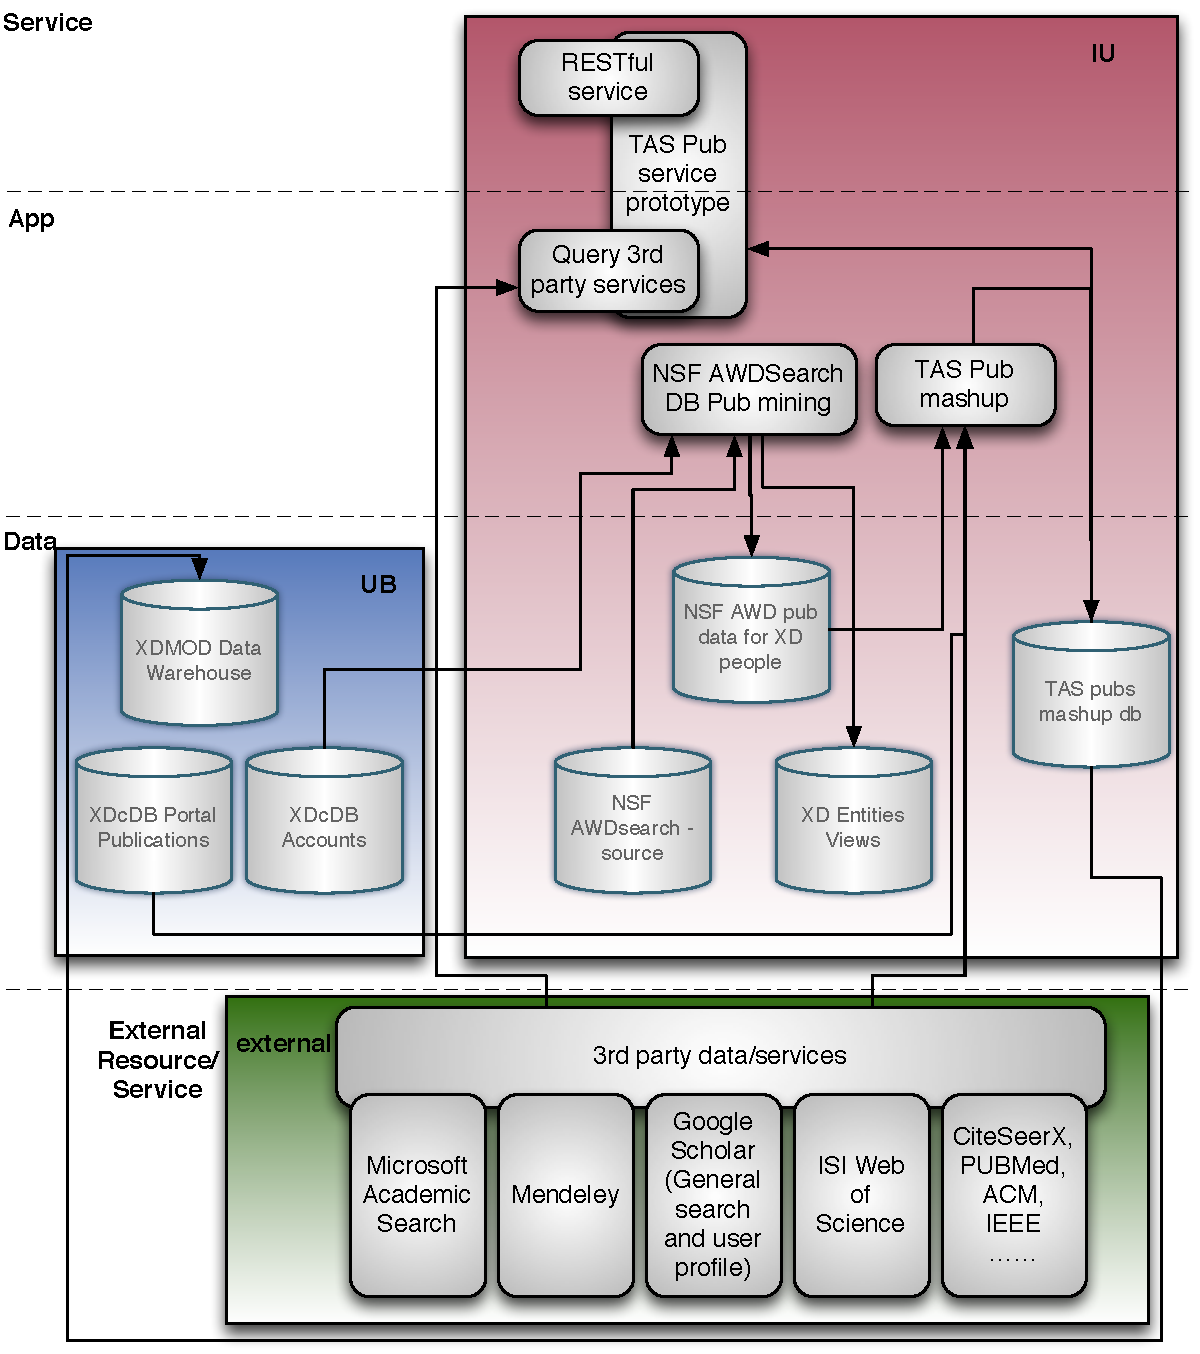
\includegraphics[width=1.0\columnwidth]{images/tas-arch.pdf} 
  \caption{The Architecture of the Framework}\label{F:tas-arch} 
\end{figure} 

We have designed a software framework to support measuring scientific impact via a publication and citation based approach. The framework is based on distributed set of services (involving Indiana University (IU), University at Buffalo (UB), National Center for Supercomputing Applications (NCSA) at the University of Illinois and other external resources). This service-oriented system consists of components for publication and citation data retrieval (e.g., from Google Scholar and ISI Web of Science), parsing and processing while correlating data from various databases and services, such as the XSEDE central database (XDcDB), which stores all usage data for jobs run on XSEDE resources, the Partnerships Online Proposal System (POPS) database, which stores publication and grant funding information for PI’s applying for an XSEDE allocation. The NSF award database is also included and represents an extensive source of publication and award information for the TeraGrid/XSEDE PI’s.  Our service orientated system also includes components for metrics generation and an analysis system for different aggregation levels (users, projects, organization, Field of Science (FOS)), as well as a presentation layer using a light weight portal in addition to exposing some data via RESTful API
 
Fig \ref{F:tas-arch} shows the layered system architecture, with an emphasis on the relationships between related components especially those integrating with databases. On the core \emph{\textbf{App}} layer we have the database mining and publication mashup components. The database mining component queries the NSF award database for each XSEDE user from the XDcDB mirror. It generates the XSEDE user specific publication data as well as user, project, and Field of Science (FOS) views. The publication mashup component aggregates the publication data mined from the previous component, as well as those from XDcDB, and from other available external services. It also retrieves citation data for each publication from external services, e.g. Google Scholar and ISI Web of Science. Another essential task of this component is to generate metrics for users, projects, and FOS in which the POPS db is involved to get proposal and project data. These data will be then stored into the mashup db which can be integrated into the XDMoD \cite{CPE:CPE2871} system at our partner site UB. We also expose some data and analysis results via RESTful API and a portal as denoted on the \emph{\textbf{Service/GUI}} layer. The \emph{\textbf{Data}} layer illustrates the databases involved, which include XDcDB mirro and XDMoD data warehouse at UB, the POPS db at NCSA, and the rest at IU. The \emph{\textbf{External Resource/Services}} layer lists the third party resource and services that we are currently using or have experimented or plan to investigate.

For this study, the general workflow is that we obtain the publication data for each XSEDE user, and then retrieve the citation data for each publication. The data is originally collected per user and per publication basis, but can also be aggregated based on organization, XSEDE project/account, FOS, and other categories while providing the input for the metrics generation and analysis. When correlating the data with the input (for example the Service Units (SUs) awarded by XSEDE) the analysis may reveal patterns and trends of how XSEDE can impact the sciences and potentially helps to achieve a better measure of return on investment (ROI) for NSF. 
 
While we are using the system to analyze the scientific impact of XSEDE, the framework itself is flexible enough that could be easily adapted to other similar systems for impact measure and analyses. 
 
 
\section{Implementation} \label{S:implementation}
 
We have implemented the system following best practices and leveraging popular tools and frameworks. The core system is developed in python using the  python libraries MySQLdb, SQLAlchemy, psycopg2 to interact with the various data sources. Python library requests and BeautifulSoup are used for scraping citation data and properly parsing them. The Flask framework is used for the service interface and Web GUI. Various JavaScript libraries such as highcharts are utilized in the Web tier. 
 
Publication and citation data retrieval was an complicated but essential part of our study, so we provide details of the process next. 
 
\subsection{Publication Data Acquisition} 
 
\begin{figure}[!htb] 
  \centering 
    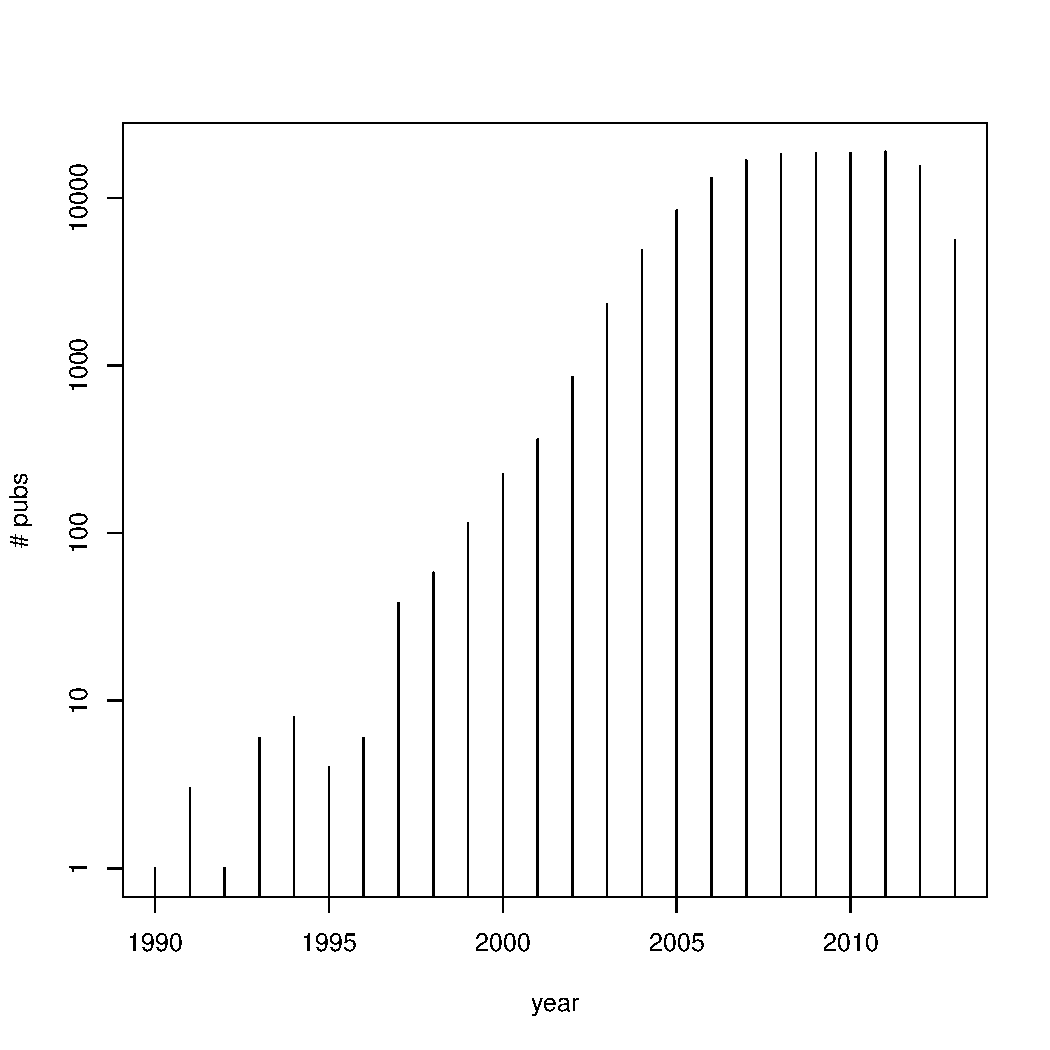
\includegraphics[width=1.0\columnwidth]{images/21_pubs_year_distribution.pdf} 
  \caption{Number of Publications Retrieved by Year}\label{F:pubs-year-distribution} 
\end{figure} 
 
\begin{figure}[!htb] 
  \centering 
    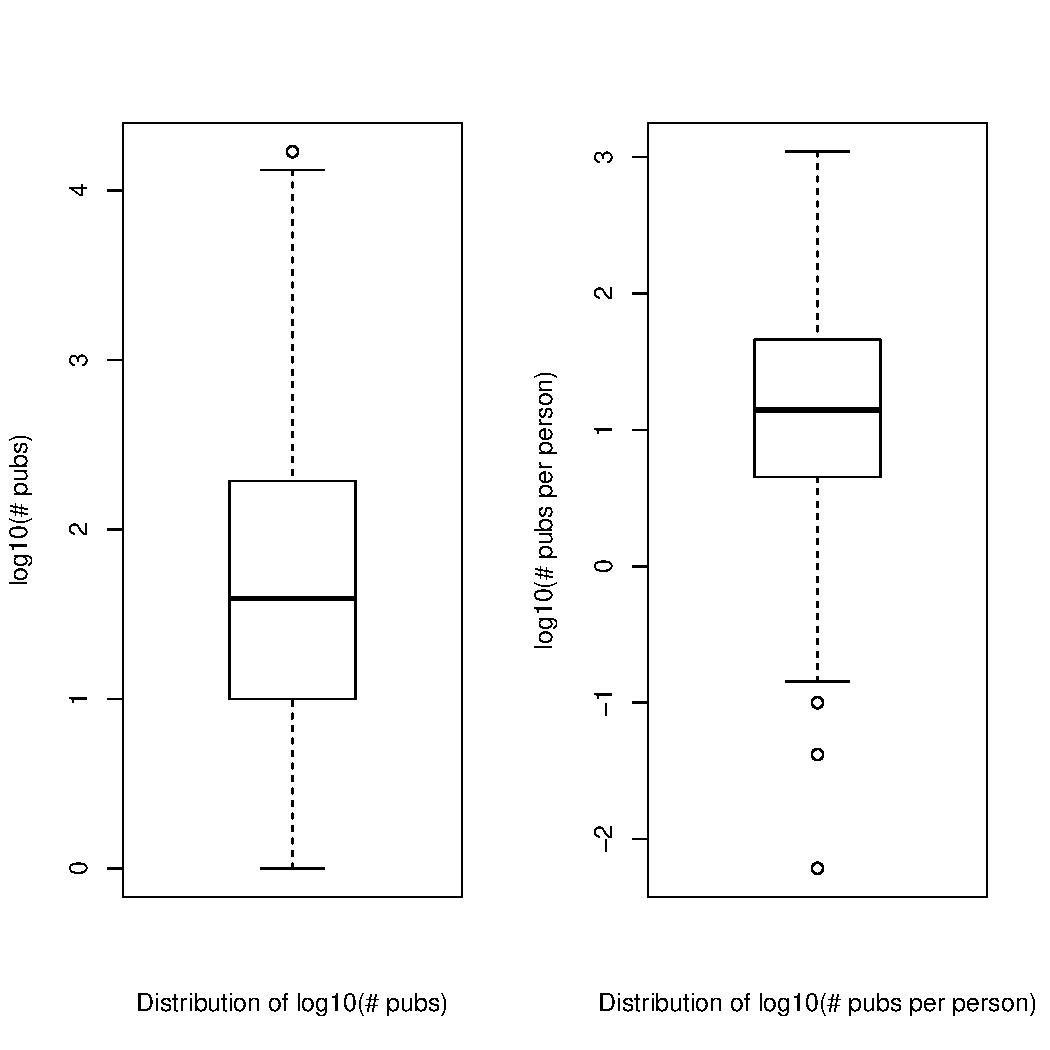
\includegraphics[width=1.0\columnwidth]{images/01_dist_npubs_proj.pdf} 
  \caption{Distribution of number of publications}\label{F:dist-npubs-proj} 
\end{figure} 
 

We started the project by following the automated approach to obtain publication data. Publication citation data are available via subscribed resources such as ISI Web of Science \cite{www-isiwos} or open access such as Google Scholar \cite{www-googlescholar}, Microsoft Academic Search \cite{www-msas}, and Mendeley \cite{www-mendeley}, however they unfortunately usually do not provide unlimited access, making automated publication retrieval impractical. 
 
Another approach is to obtain the publication data directly from users. As the user curated data it tends to be more accurate in comparision to automated publication mining. Additionally, it can provide extra information regarding a publication's association with the system, e.g., to which project it belongs. 
Such a system was first implemented in FutureGrid leveraging the drupal biblio module \cite{www-drupal-bib} which we customized to support easy publication reporting and mass publication imports directly by the users. This upload is correlated with the project the publication is most closely related to \cite{www-fgbiblio}. XSEDE replicated this functionality and now provides it via their XSEDE portal \cite{www-xdportalpub} using a different portal framework. The nanoHub citation analysis \cite{www-nanohubcite} as we have mentioned is also based on publication data submitted by users via a web form. 
 
The framework reported on in this paper supports pluggable data sources that allow for the mining of databases and/or accessing 3rd party service APIs. We have experimented with various data sources including Microsoft Academic Search, Google Scholar including user profiles, and mining the extensive NSF award database that is available upon request from NSF. The extracted data records are then stored into our Mashup database that provides a common interface to other components in the system as well as collaborating systems like XDMoD \cite{CPE:CPE2871}. 
 
In this study we focus only on two of these data sources - the user submitted data via the XSEDE portal, and the extensive NSF award database for automated mining. The former source has user curated data with project affiliation information, and thus in principal it gives a measure of \emph{direct} impact of XSEDE. However, since this system of self reporting has only been in existence for little more than a year through the XSEDE users portal, is has very limited data entries.  On the other hand, the NSF award database contains an extensive compilation of publications that can be automatically mined to pull out all publications for a given XSEDE user.   While we cannot directly correlate the publications obtained in this way with XSEDE resources, it does nonetheless provide a measure on a general or \emph{indirect} impact of XSEDE.   As a given XSEDE user is affiliated with accounts/projects, and the projects are part of one or more FOS, we can thus tag a publication as being related to the projects and FOS's based on these indirect correlations. Although not ideal, it provides a means to analyze the \emph{indirect} impact. 
 
Based on this technique, we have been able to obtain over 142,000 publication entries for over 20,000 XSEDE users as of Jan 2014.  This by itself is substantial accomplishment and as we know of no other database that has this level of detail that can be correlated to researcher's participating in XSEDE. To provide a quick overview of the data analyzed we refer to Figure \ref{F:pubs-year-distribution} showing the yearly distribution of the publications. Figure \ref{F:dist-npubs-proj} shows the distribution of number of the publications by project (on the left) and by per user for each project. 
 
\subsection{Citation Data Retrieval} 
 
While for the publication data the user curated data might be more ideal, we need to conduct an automated search to identify the subsequent citations of the publication recovered from the NSF award database. 
Due to the size of this publication data (142,000 publications), the only realistic way to accomplish this is with an automated process. Google Scholar and ISI Web of Science provide such data but with some noticeable limitations. In case of Google Scholar the API is not provided, nor does it allow unlimited access within a bounded time period from one request source.\footnote{Please note that the API and access used to be available, but has been removed from public access for a while now. While previous efforts could benefit from this today the limitation provides a significant hurdle.} ISI data does not impose a rate limiting while you have subscribed access, however it does also not provide an easy access API. Thus we were forced to emulate such an API while submitting queries via the web UI and then parse the data from the tabulated results list. 
 
In order to compare the two methods of obtaining citations, we explored Google Scholar and ISI data for a subset of the publication data, and did a comparison of the results. While a similar comparison has been attempted \cite{yang2006citation}, it was restricted to a very small sample size - 2 people and about 100 publications. In comparison, our study included 33,861 publications and 1,462 users, moreover they are related to XSEDE.
 
\begin{figure}[!htb] 
  \centering 
    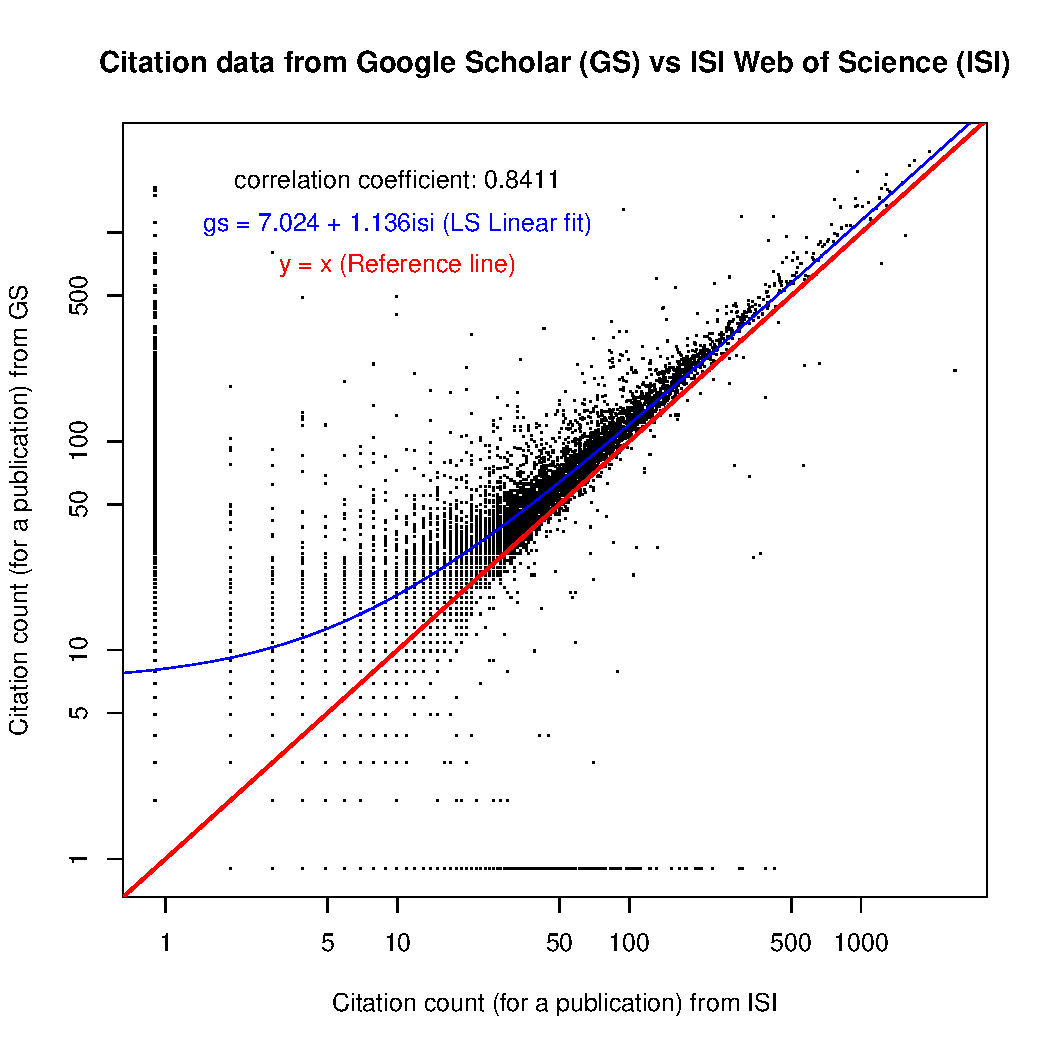
\includegraphics[width=1.0\columnwidth]{images/11_gs_vs_isi_cites.pdf} 
  \caption{Citation counts comparison for a subset of our publication data}\label{F:gs-vs-isi-cites} 
\end{figure} 
 
\begin{figure}[!htb] 
  \centering 
    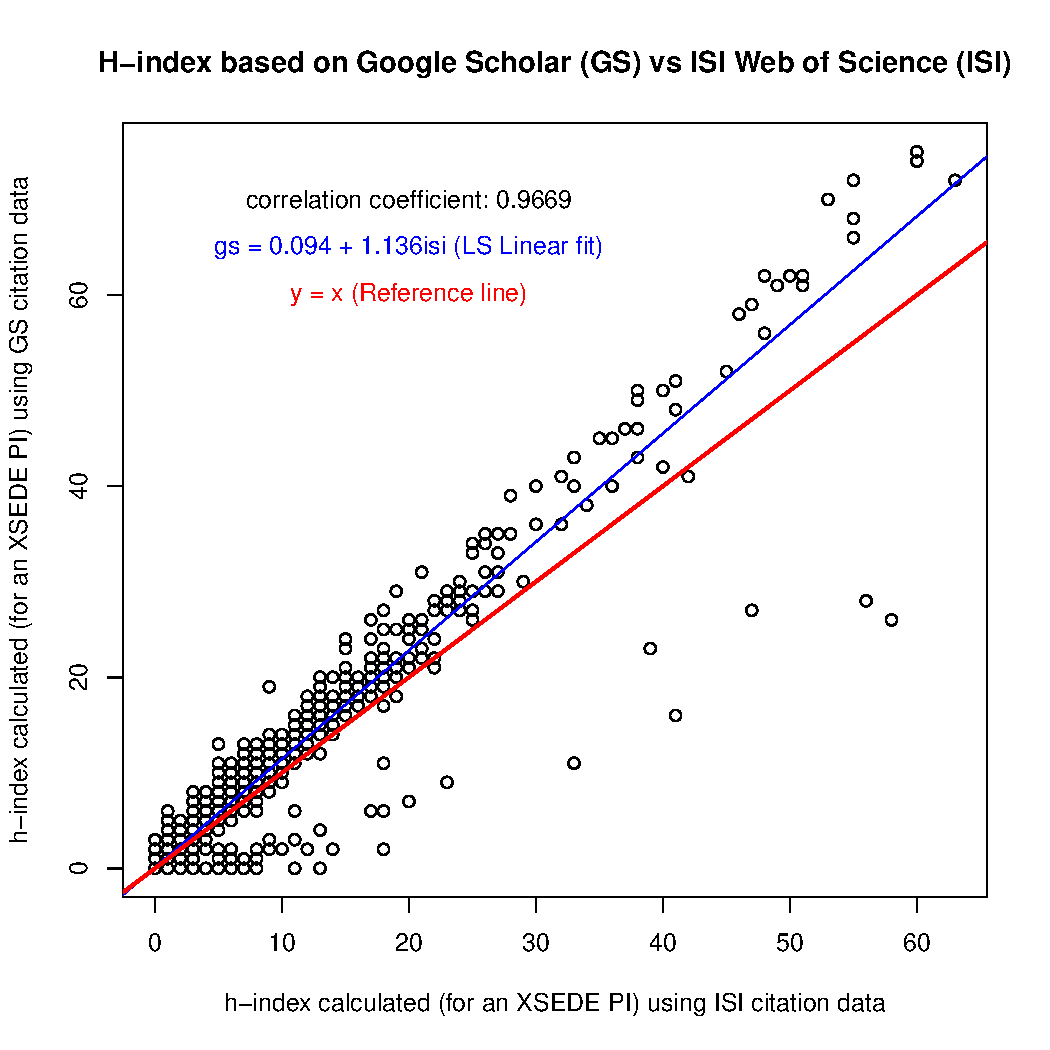
\includegraphics[width=1.0\columnwidth]{images/11_gs_vs_isi_hindex.pdf} 
  \caption{H-index comparison for a subset of XSEDE PIs}\label{F:gs-vs-isi-hindex} 
\end{figure} 
 
The result of this activity is depicted in Figure \ref{F:gs-vs-isi-cites} and correlates the citation data from Google Scholar (GS) with the ISI Web of Science. Out of the 33861 data points, 20793 of them (61.4\%) have larger values in GS, 10315 (30.5\%) are the same, while 2753 (8.1\%) have larger values in ISI. 5287 (15.6\%) publications have zero citation found in ISI but non-zero in GS, 1253 (3.7\%) pubs have zero citation in GS but non-zero in ISI. Thus we conclude that in general Google Scholar tends to have higher citation number. 
 
Figure \ref{F:gs-vs-isi-hindex} shows that h-index obtained from Google Scholar data and correlates it to data from ISI. Out of the 1462 data points, 663 of them (45.3\%) have larger value in GS, 677 (46.3\%) are the same, while 122 (8.3\%) have larger value in ISI. 52 (3.6\%) PIs have zero h-index computed from ISI data but are non-zero in GS, 39 (2.7\%) for the reverse side. Thus we conclude that in general the h-index calculated from Google Scholar data tends to be a bit higher. 
 
In either case a high positive correlation is observed. The Pearson correlation coefficient are 0.84 and 0.97 respectively. The very strong correlation of the h-index values are mostly due to the fact that one of the two factors determining the h-index, the number of publications, stay the same for a particular user. 
 
Based on our study while being aware of the limitations, we were able to use the ISI citation data to get very similar measures for most of the data especially for the h-index metric. This is especially useful if we consider that we do have issues to retrieve a complete citation data set from Google scholar for each of our relevant users and publications.

Thus the following analyses are only using citations from ISI to further derive other metrics. 
 
\section{Results and Analyses} \label{S:result}
 
The previous section described the method used to extract publication and citation data for XSEDE users.  With this data now in hand, we discuss the metrics derived from this data with the goal of providing a measure of scientific impact. We will also conduct analyses to determine if a correlation exists between the data and various categories such as field of science. 
 
\subsection{Direct impact of XSEDE} 
 
\begin{figure*}[!htb] 
  \centering 
    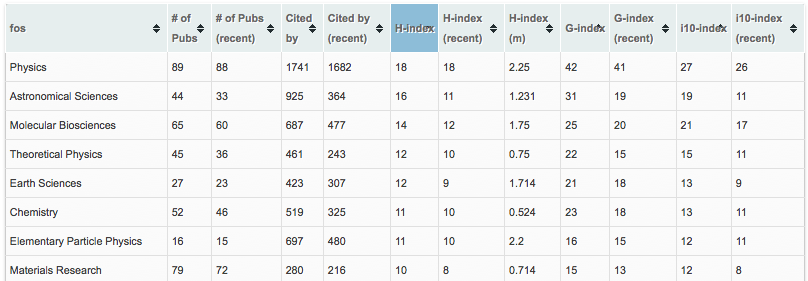
\includegraphics[width=2.0\columnwidth]{images/XDPUBS_Metrics_FOS.png} 
  \caption{Impact metrics for top FOS sorted by h-index (based on currently available data as of Jan 2014)}\label{F:xdpubs-metrics-fos} 
\end{figure*} 
 
By using the user vetted submitted publications only\footnote{which are tagged as \emph{direct} output of XSEDE projects}, we were able to show the \emph{direct} scientific impact of XSEDE.  As of Jan 27, 2014, there are currently registered 837 publications involving 882 XSEDE users as authors, 220 organizations, 331 XSEDE projects, and a total of 11,258 citations to date. Please note that these values are temporarily and that they are incomplete as not all users have contributed their publications to XSEDE projects.   This will change however, as the XSEDE's revised allocation request process will now dramatically improve the ease at which users can upload their publication information.

Based on this data, we calculated the various metrics on the level of user, organization, projects, and FOS involved. Figure \ref{F:xdpubs-metrics-fos} shows the FOS's judging with the highest h-index values. 
 
\subsection{Project metrics vs SUs allocation} 
 
\begin{figure}[!htb] 
  \centering 
    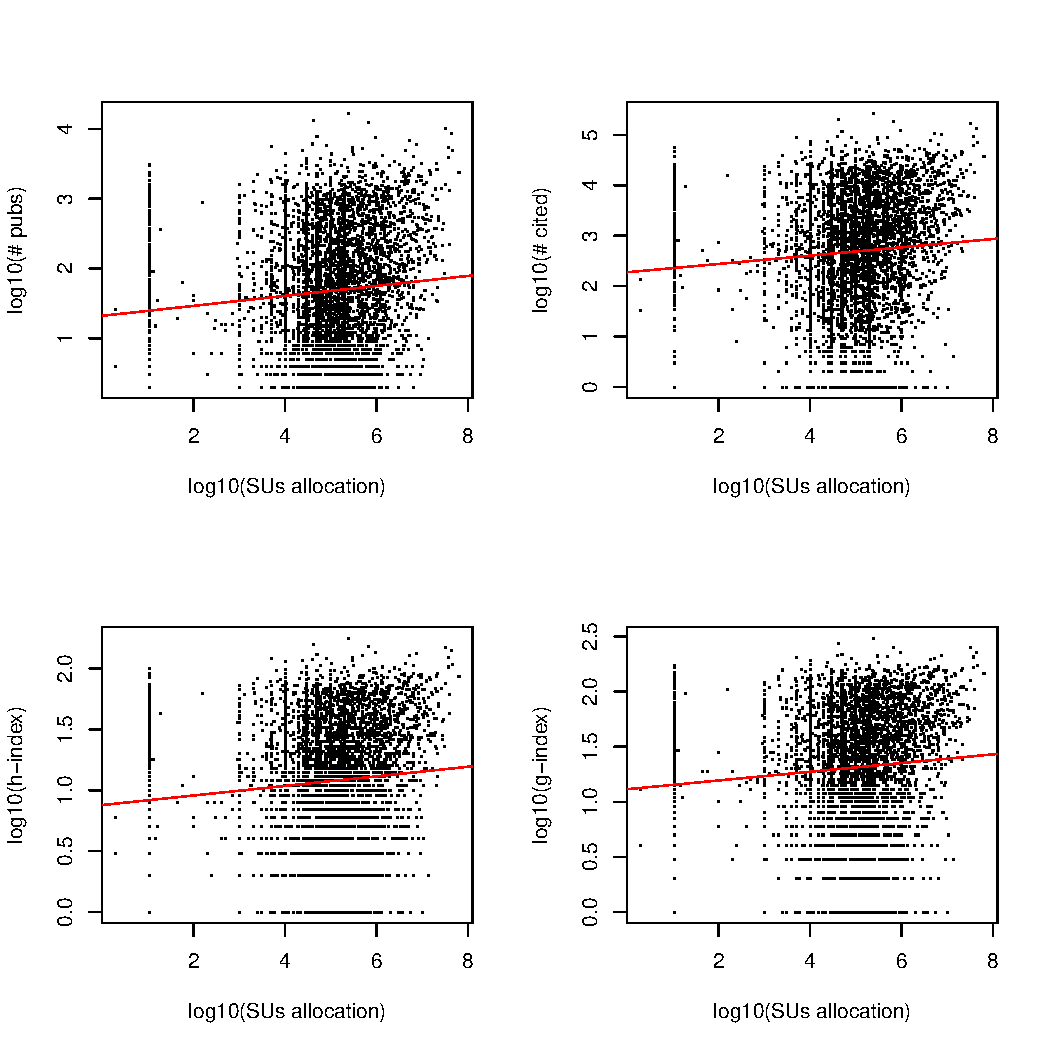
\includegraphics[width=1.0\columnwidth]{images/02_metrics_vs_alloc_proj.pdf} 
  \caption{Impact Metrics (number of publications, number of citations, h-index, g-index) vs SUs for all projects}\label{F:metrics-vs-alloc-proj} 
\end{figure} 
 
\begin{figure}[!htb] 
  \centering 
    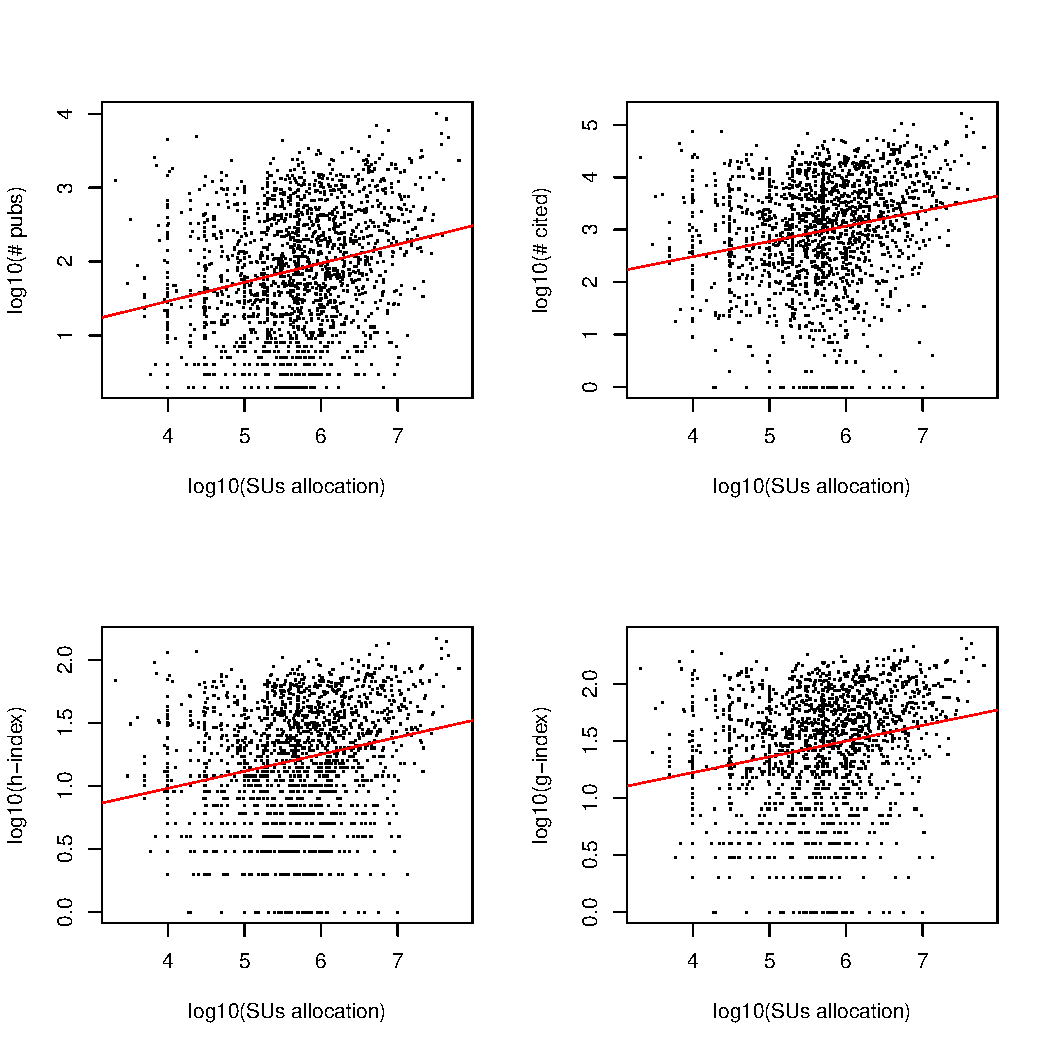
\includegraphics[width=1.0\columnwidth]{images/02_metrics_vs_alloc_research_proj.pdf} 
  \caption{Impact Metrics (number of publications, number of citations, h-index, g-index) vs SUs for research projects}\label{F:metrics-vs-alloc-research-proj} 
\end{figure} 
 
%\begin{figure}[!htb] 
%  \centering 
%    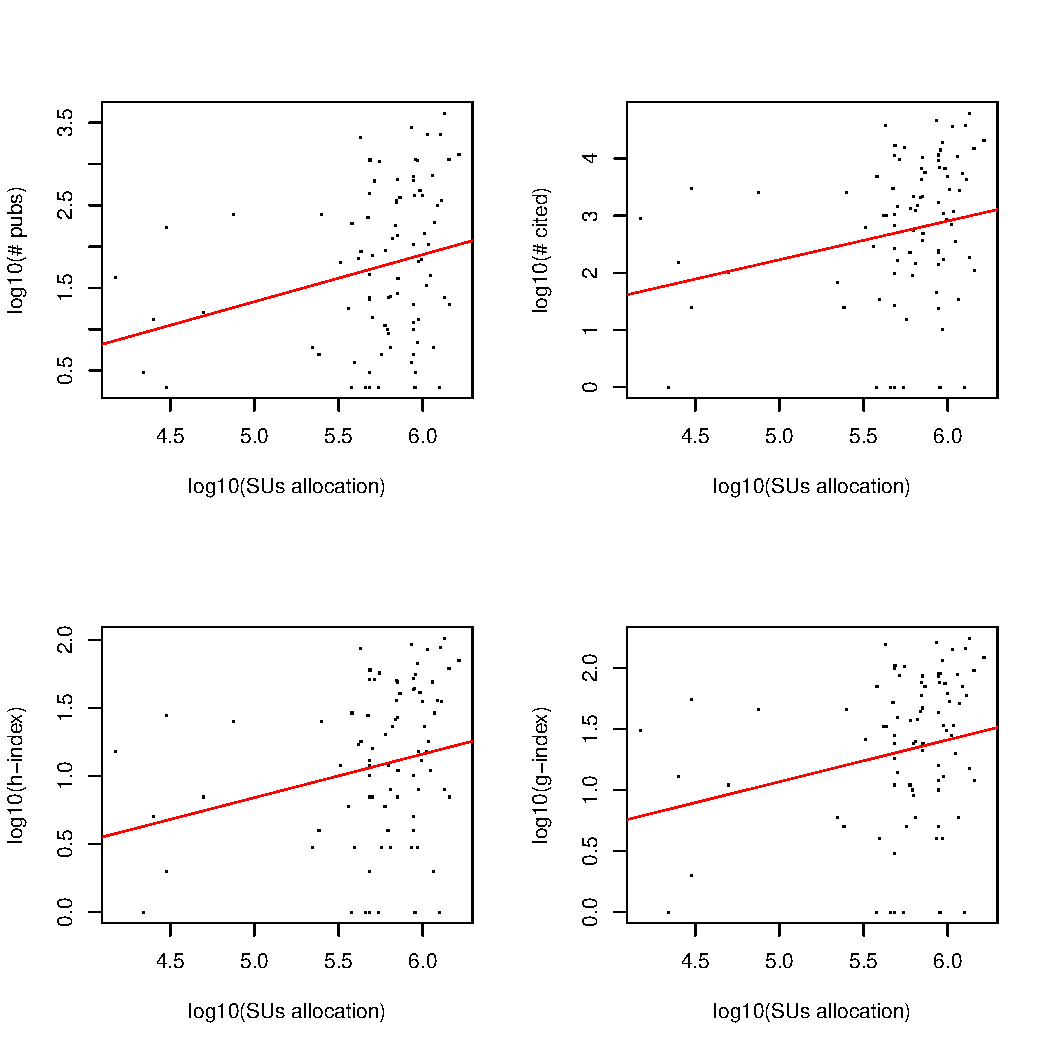
\includegraphics[width=1.0\columnwidth]{images/02_metrics_vs_alloc_campus_proj.pdf} 
%  \caption{Metrics vs SUs for campus champion projects}\label{F:metrics-vs-alloc-campus-proj} 
%\end{figure} 
 
%\begin{figure}[!htb] 
%  \centering 
%    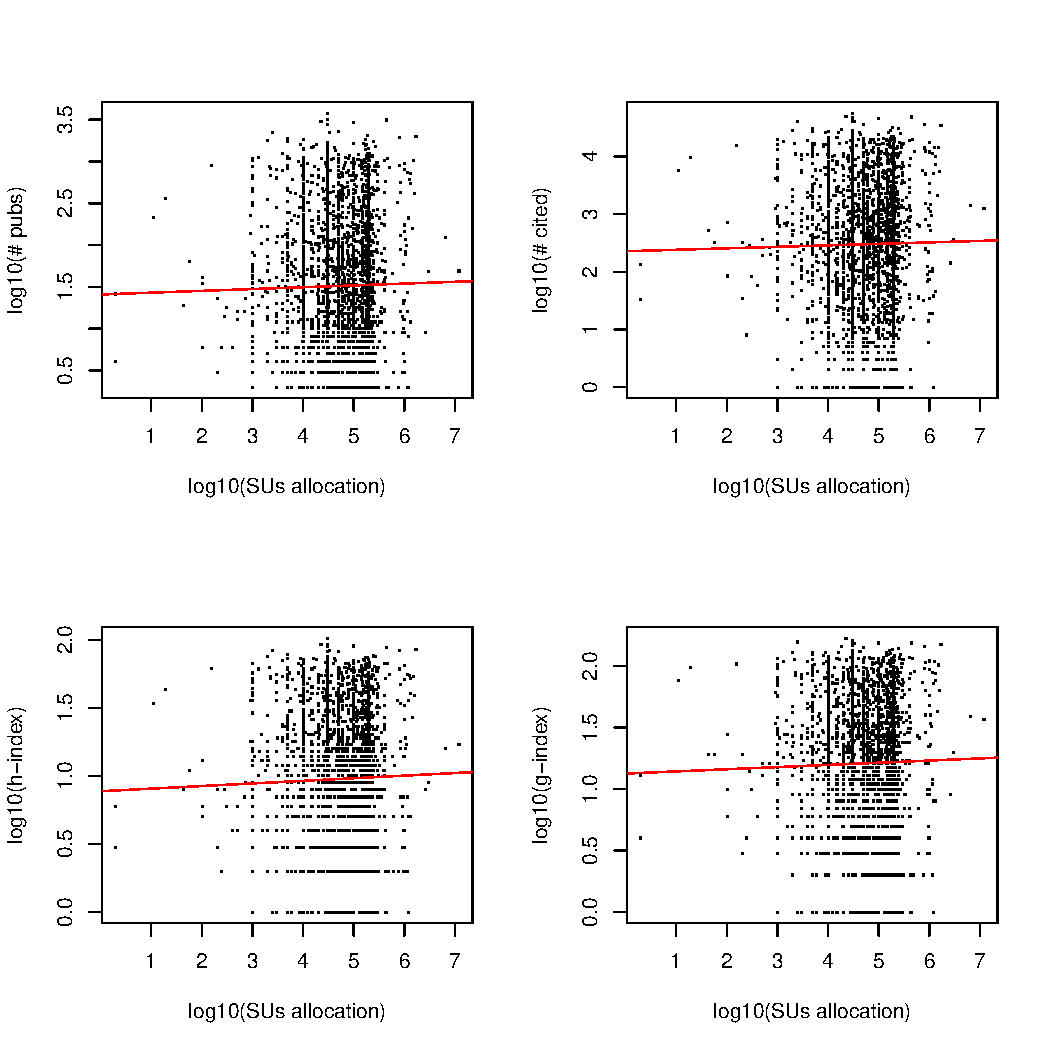
\includegraphics[width=1.0\columnwidth]{images/02_metrics_vs_alloc_startup_proj.pdf} 
%  \caption{Metrics vs SUs for startup projects}\label{F:metrics-vs-alloc-startup-proj} 
%\end{figure} 
 
\begin{table}[!htb] 
  \centering 
    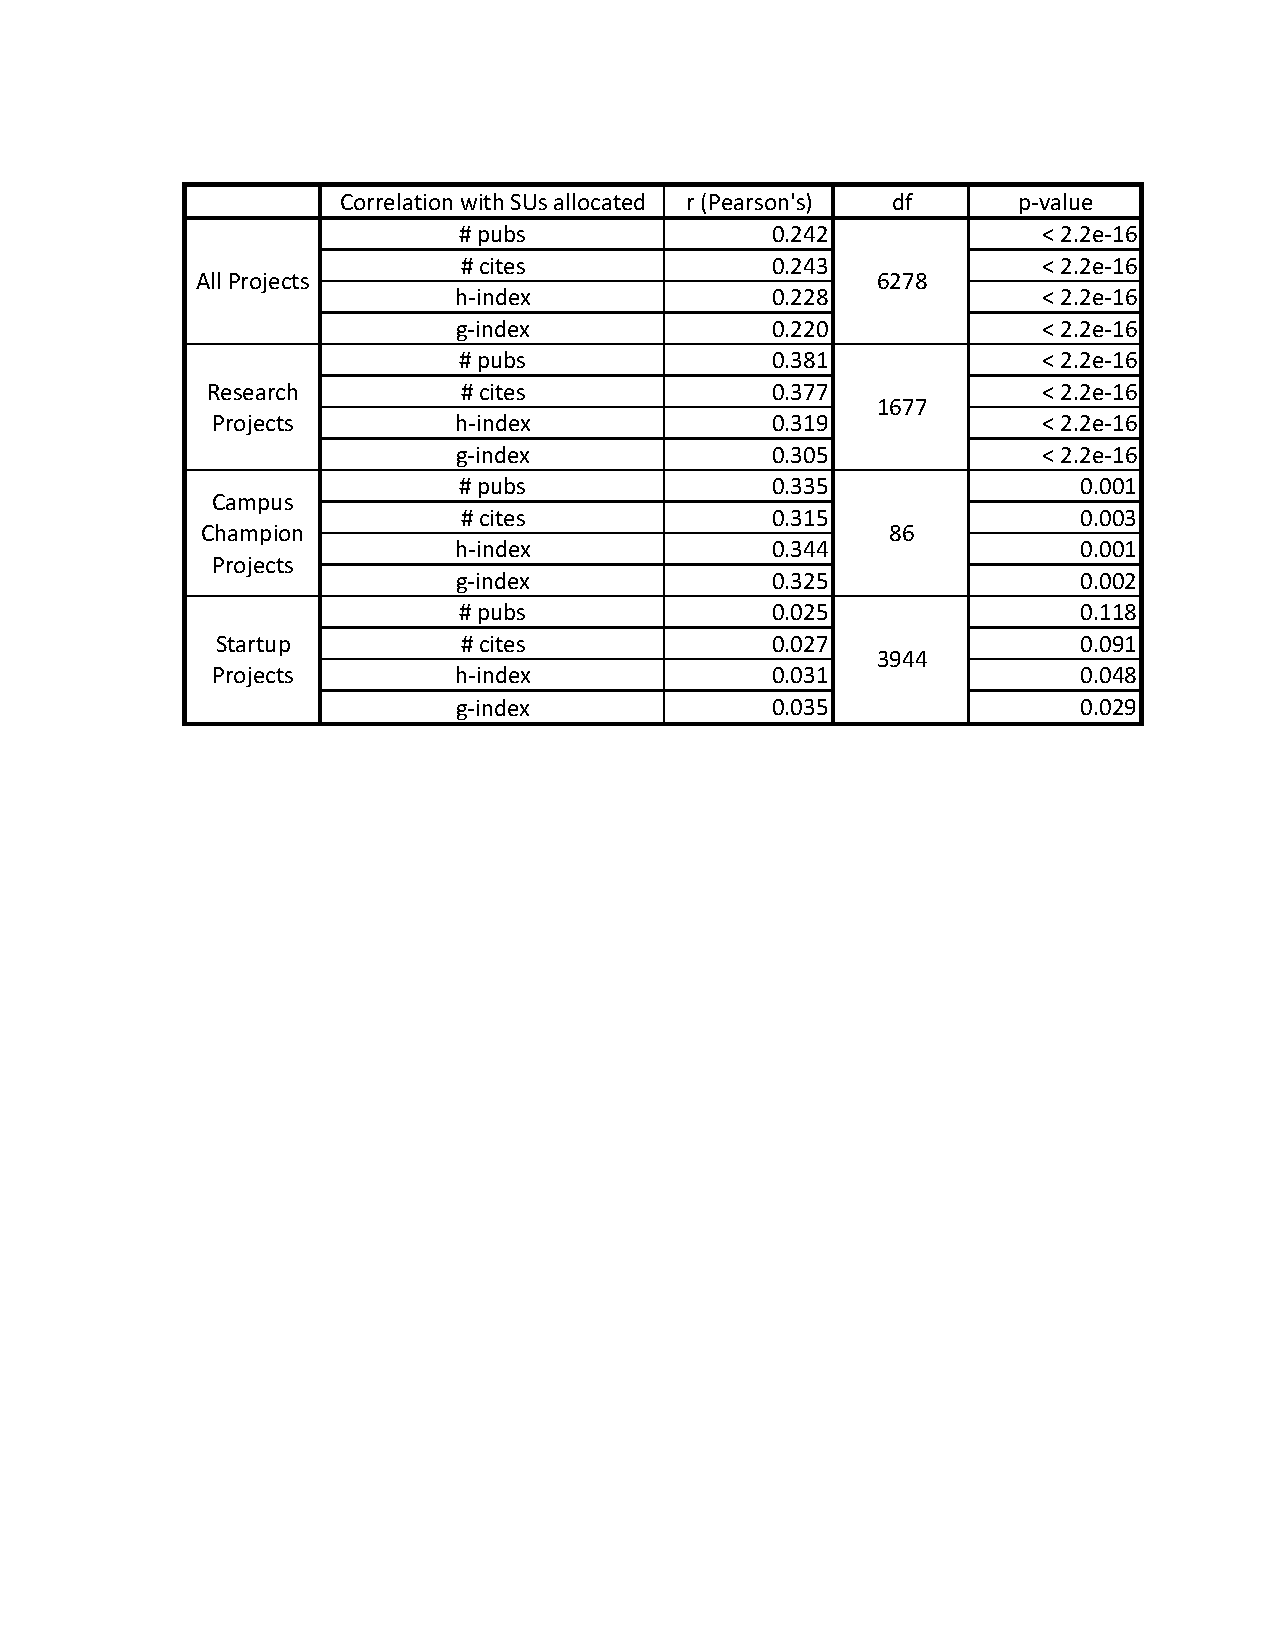
\includegraphics[width=1.0\columnwidth]{images/metrics_alloc_r.pdf} 
  \caption{Correlation between SUs allocated vs the impact metrics for each project}\label{F:metrics-alloc-r} 
\end{table} 
 
Figure \ref{F:metrics-vs-alloc-proj} shows the correlation analysis of impact metrics (number of publications, number of citations, h-index, and g-index) versus XD resource allocation (number of SU's) for an individual project (research, start-up, campus champion, etc).  Previous work showed a stronger correlation between the citation and SUs \cite{bollen2011and} using a much smaller sample size taken from a specific XSEDE resource allocation meeting. However, we observed a weaker correlation, if any. When categorizing the projects based on the types (research, startup, campus champion, etc.), it shows a slighty stronger correlation,  although still not as strong in correlation to each category other than for the startup projects/allocations. Figure \ref{F:metrics-vs-alloc-research-proj} shows the analysis for research projects only. Table \ref{F:metrics-alloc-r} lists the correlation coefficient values as well as the p-values showing the significance of the test. Please note in Figure \ref{F:metrics-vs-alloc-proj} and \ref{F:metrics-vs-alloc-research-proj} we included a regression line showing the upper trends of the correlation, i.e., higher SUs allocation correlating to higher impact metrics, but not suggesting a linear relationship. This correlation analysis does not show the cause effect either, as in this case it is very likely that the causal are reciprocal. 
 
\subsection{Metrics vs SUs allocation on FOS level} 
 
\begin{figure}[!htb] 
  \centering 
    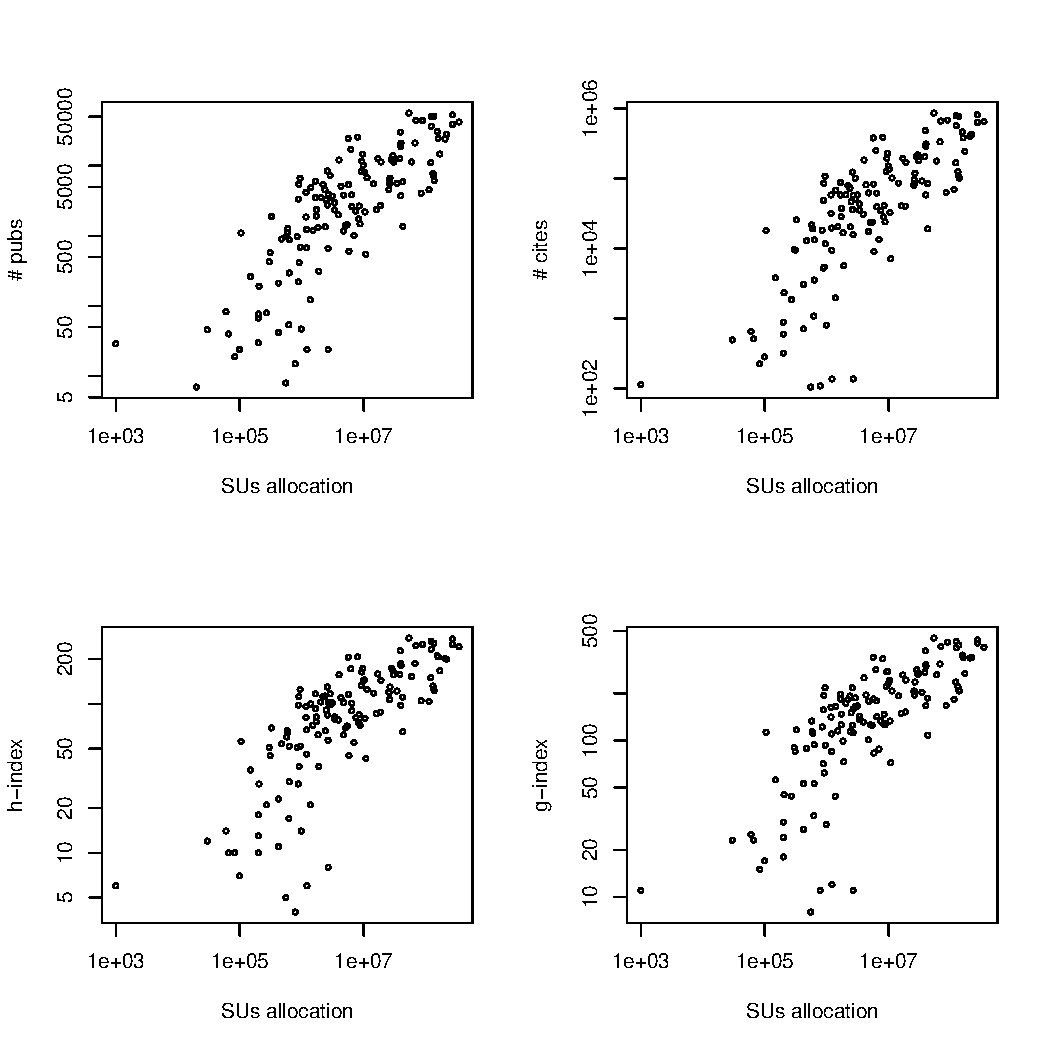
\includegraphics[width=1.0\columnwidth]{images/03_metrics_vs_alloc_fos.pdf} 
  \caption{Impact Metrics (number of publications, number of citations, h-index, g-index) vs SUs for FOS's}\label{F:metrics-vs-alloc-fos} 
\end{figure} 

While on an individual project level we do not observe strong correlations between impact metrics (number of publications, number of citations, h-index, and g-index) and the resource allocations, Figure \ref {F:metrics-vs-alloc-fos} shows stronger positive correlation on the FOS category. The Pearson correlation coefficient are 0.704, 0.712, 0.651, 0.648 respectively for the four impact metrics - number of publications, number of citations, h-index and g-index. With a degree of freedom at 132 and p-values less than 2.2e-16 from the test, it shows very high statistical significance.  
 
%\begin{figure}[!htb] 
%  \centering 
%    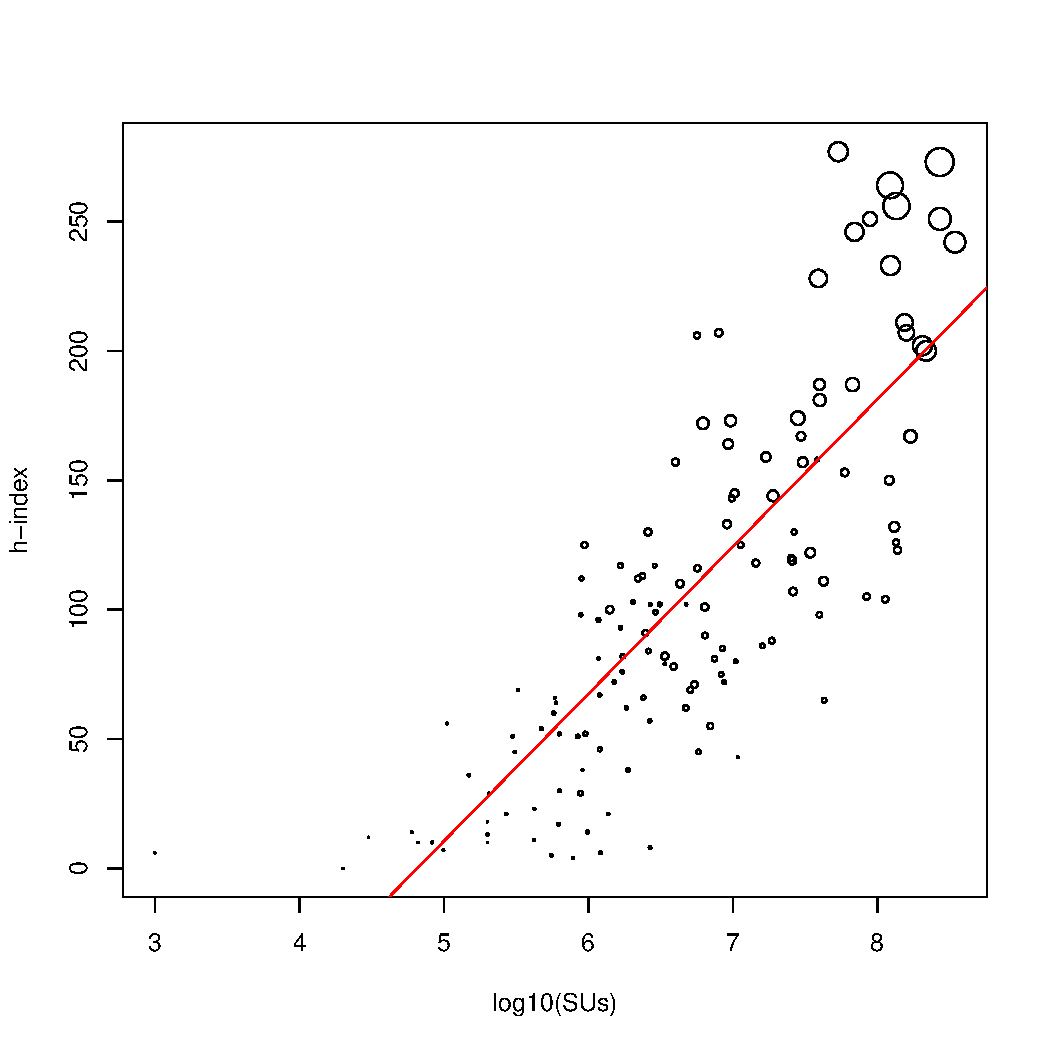
\includegraphics[width=1.0\columnwidth]{images/04_hindex_vs_alloc_fos_sized.pdf} 
%  \caption{h-index (sized by size of FOS) vs allocation}\label{F:hindex-vs-alloc-fos-sized} 
%\end{figure} 
 
\begin{figure}[!htb] 
  \centering 
    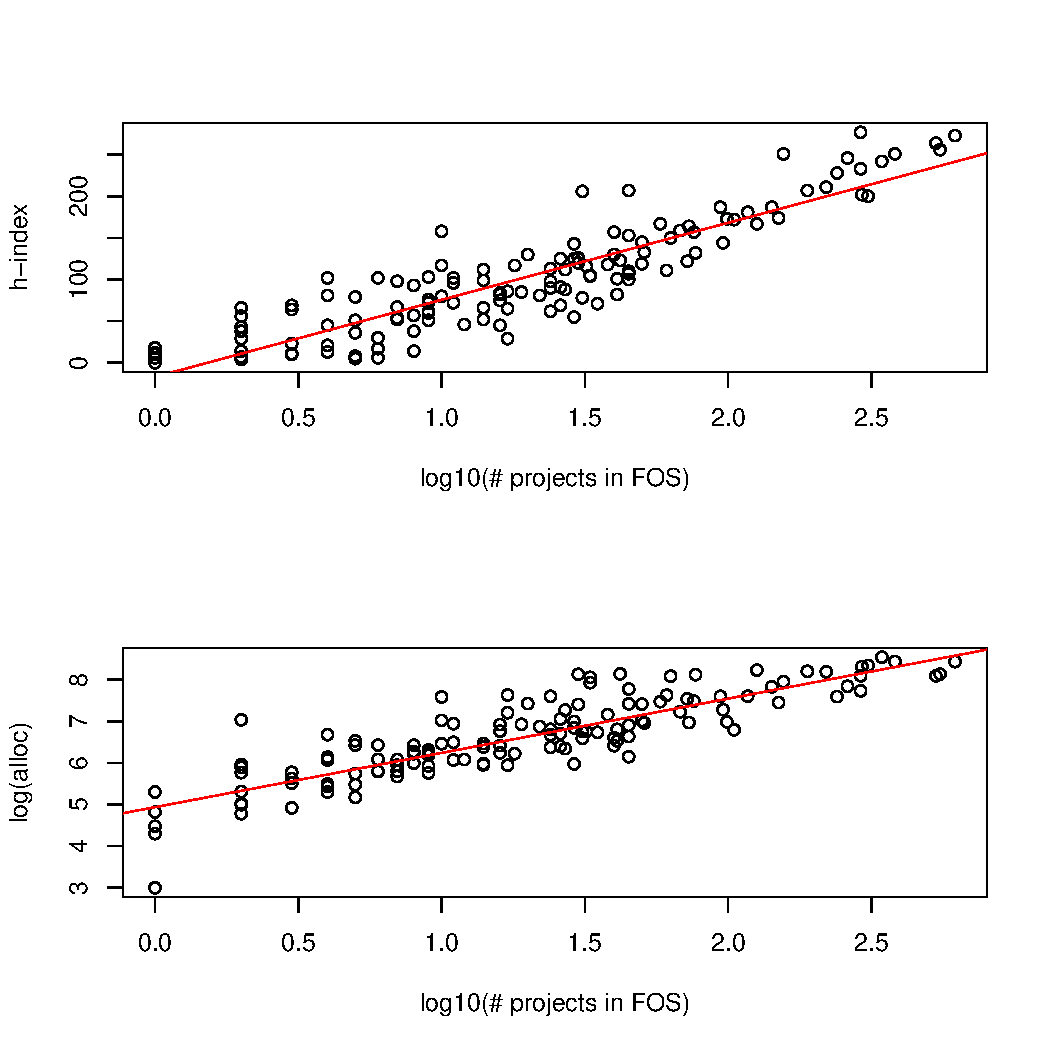
\includegraphics[width=1.0\columnwidth]{images/05_hindexalloc_vs_nprojects_fos_trended.pdf} 
  \caption{Effects of sizes of FOS's}\label{F:hindexalloc-vs-nprojects-fos-trended} 
\end{figure} 
 
However as Figure \ref{F:hindexalloc-vs-nprojects-fos-trended} suggests, the stronger correlations are mostly caused by the effect of different size of the FOS's, judging by number of projects each FOS has. However, this does not diminish the purpose of the analysis showing how XSEDE impacts science from different disciplines, e.g., by approving more projects and granting more allocations for certain FOS's. 
 
\begin{figure}[!htb] 
  \centering 
    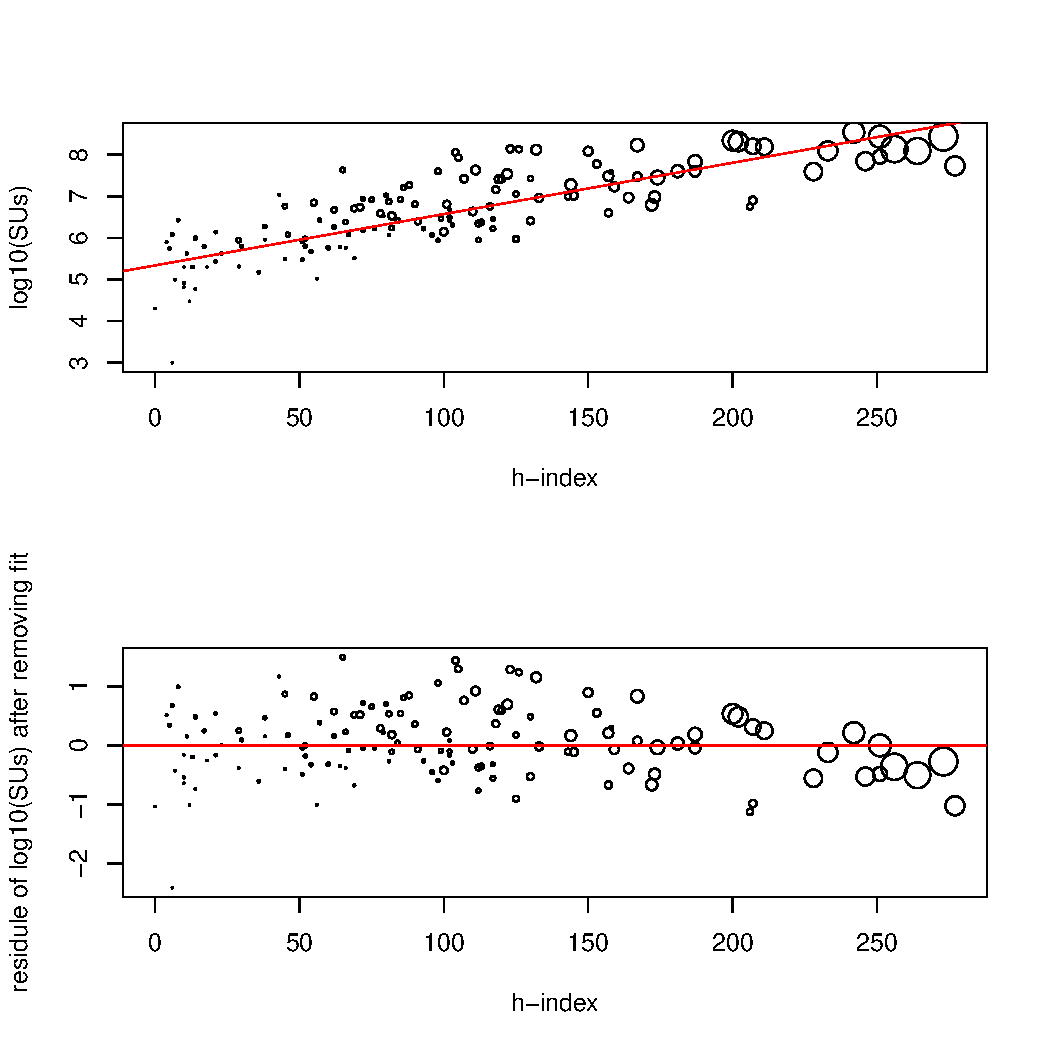
\includegraphics[width=1.0\columnwidth]{images/05_alloc_vs_hindex_fos_sized_2in1.pdf} 
  \caption{SUs vs h-index for each FOS with trend (above) and residual analysis (bottom)}\label{F:alloc-vs-hindex-fos-sized} 
\end{figure} 
 
%\begin{figure}[!htb] 
%  \centering 
%    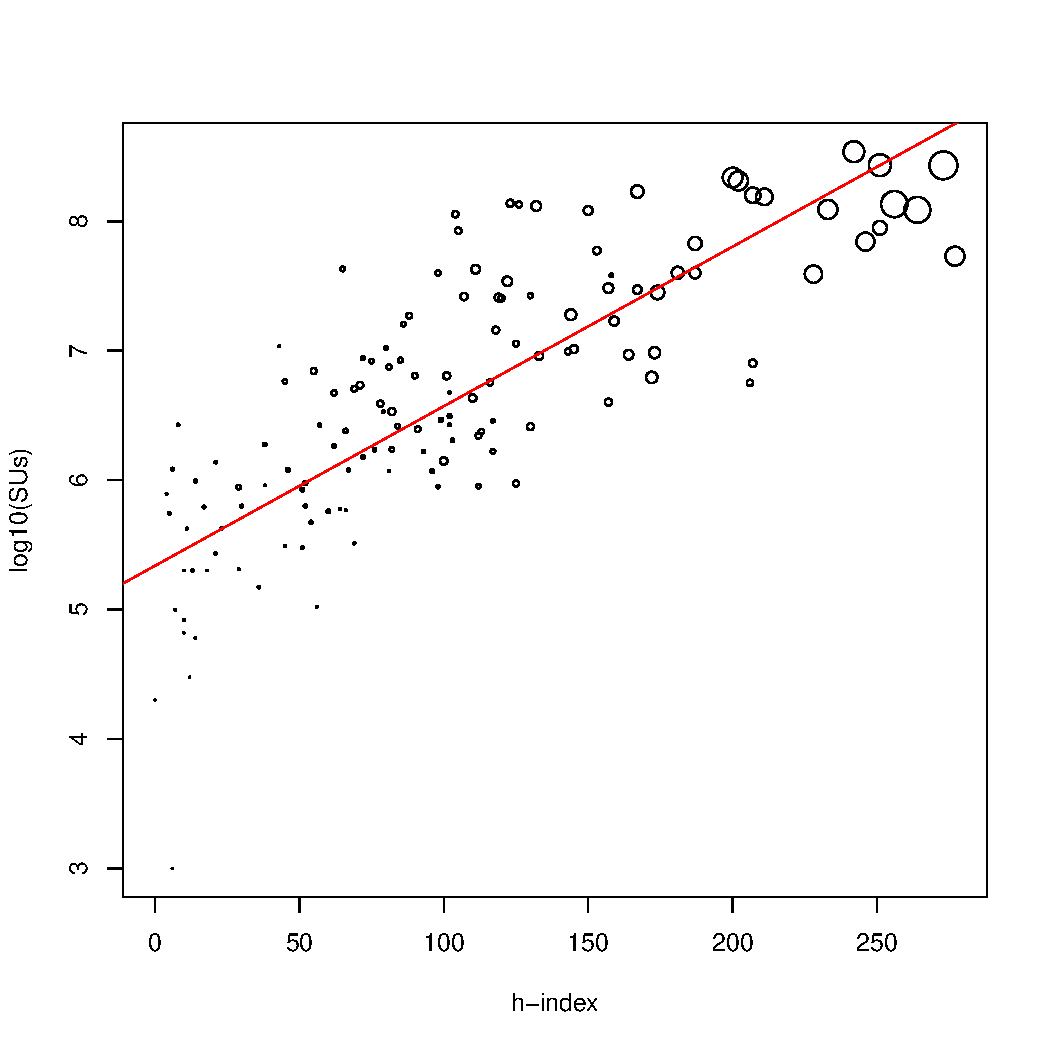
\includegraphics[width=1.0\columnwidth]{images/05_alloc_vs_hindex_fos_sized_trended.pdf} 
%  \caption{SUs vs h-index for each FOS with trend}\label{F:alloc-vs-hindex-fos-sized-trended} 
%\end{figure} 
 
%\begin{figure}[!htb] 
%  \centering 
%    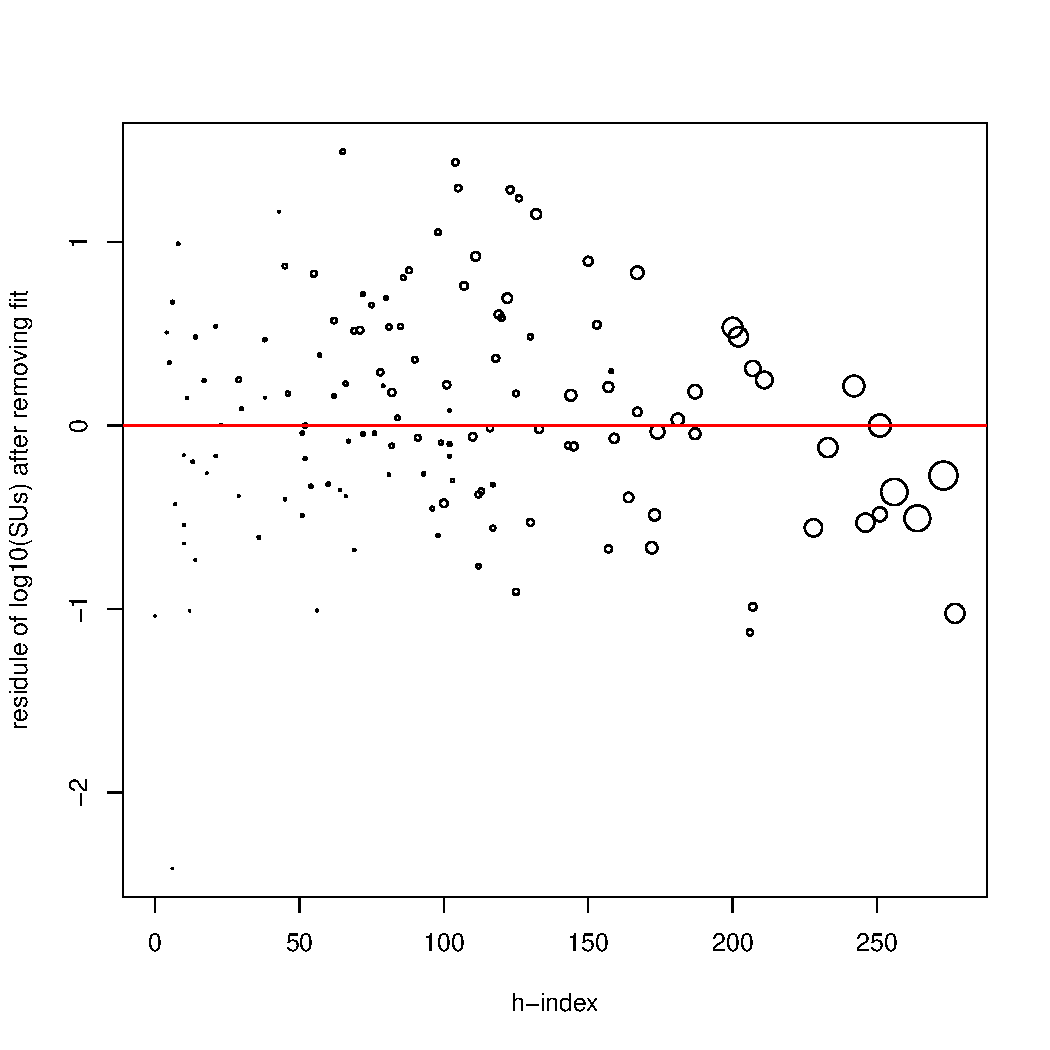
\includegraphics[width=1.0\columnwidth]{images/05_alloc_vs_hindex_fos_sized_residual.pdf} 
%  \caption{Residual analysis of SUs vs h-index}\label{F:alloc-vs-hindex-fos-sized-residual} 
%\end{figure} 
 
\begin{figure}[!htb] 
  \centering 
    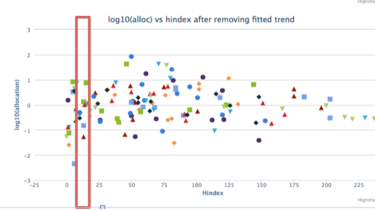
\includegraphics[width=1.0\columnwidth]{images/fig3.pdf} 
  \caption{Interactive SUs vs h-index on FOS level showing in our development portal}\label{F:fig3} 
\end{figure} 
 
Figure \ref{F:alloc-vs-hindex-fos-sized} shows the SUs allocated (transformed in logarithmic scale) vs the h-index produced for each FOS, while the circle size is proportional to the size (number of projects) of the FOS. It also shows that after removing the fitted trend, we can see a divergence of the SUs received, from the expected SUs trend to produce the given impact judging by h-index. This could imply that certain FOS's are more likely to produce a given impact while some others require more than expected SUs to produce the same impact. To further facilitate this analysis, we provided an interactive version of the plot in our web portal \cite{www-tasdeviu} and depict a screenshot in Figure \ref{F:fig3}. Through this interactive diagram we can make the following observations: 
 
\begin{enumerate} 
 
\item We can compare several FOS with the similar h-index and can easily identify some that use fewer resources than others showing a better relative output measured by the h-index. This is done by comparing FOS on a vertical slice of the h-index as annotated in Figure \ref{F:fig3} 
 
\item The trend introduces a baseline of 0. FOS above 0 use more resources than the trend, FOS bellow 0 use less resources to produce the expected impact based on a given h-index. 
 
\item Some outliers might need more careful investigation, e.g., should more or less resources be given to projects in that FOS? 
 
\end{enumerate} 
 
\begin{figure}[!htb] 
  \centering 
    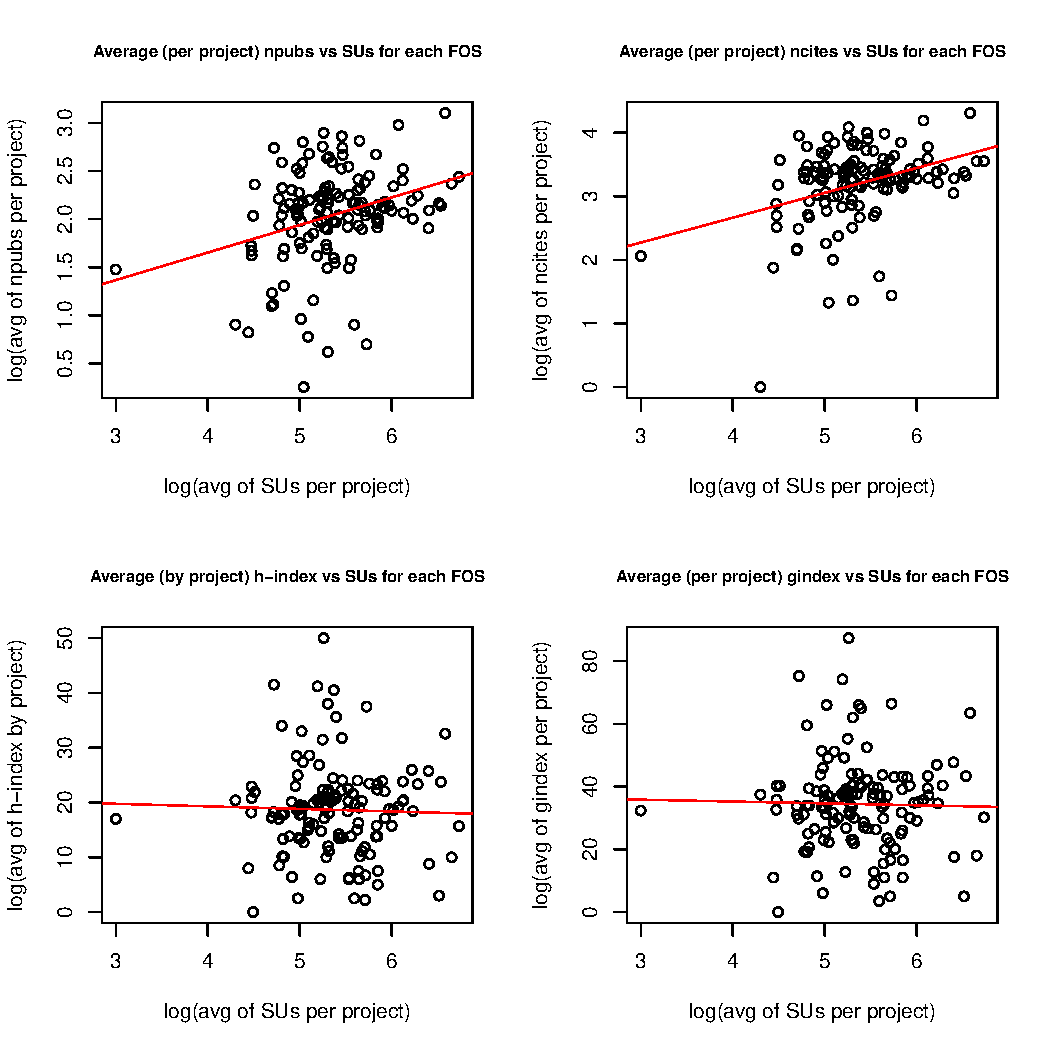
\includegraphics[width=1.0\columnwidth]{images/08_metrics_vs_alloc_avg_log_fit.pdf} 
  \caption{Impact Metrics (number of publications, number of citations, h-index, g-index) vs SUs for FOS (avg by project)}\label{F:metrics-vs-alloc-avg-log-fit} 
\end{figure} 
 
\begin{table}[!htb] 
  \centering 
    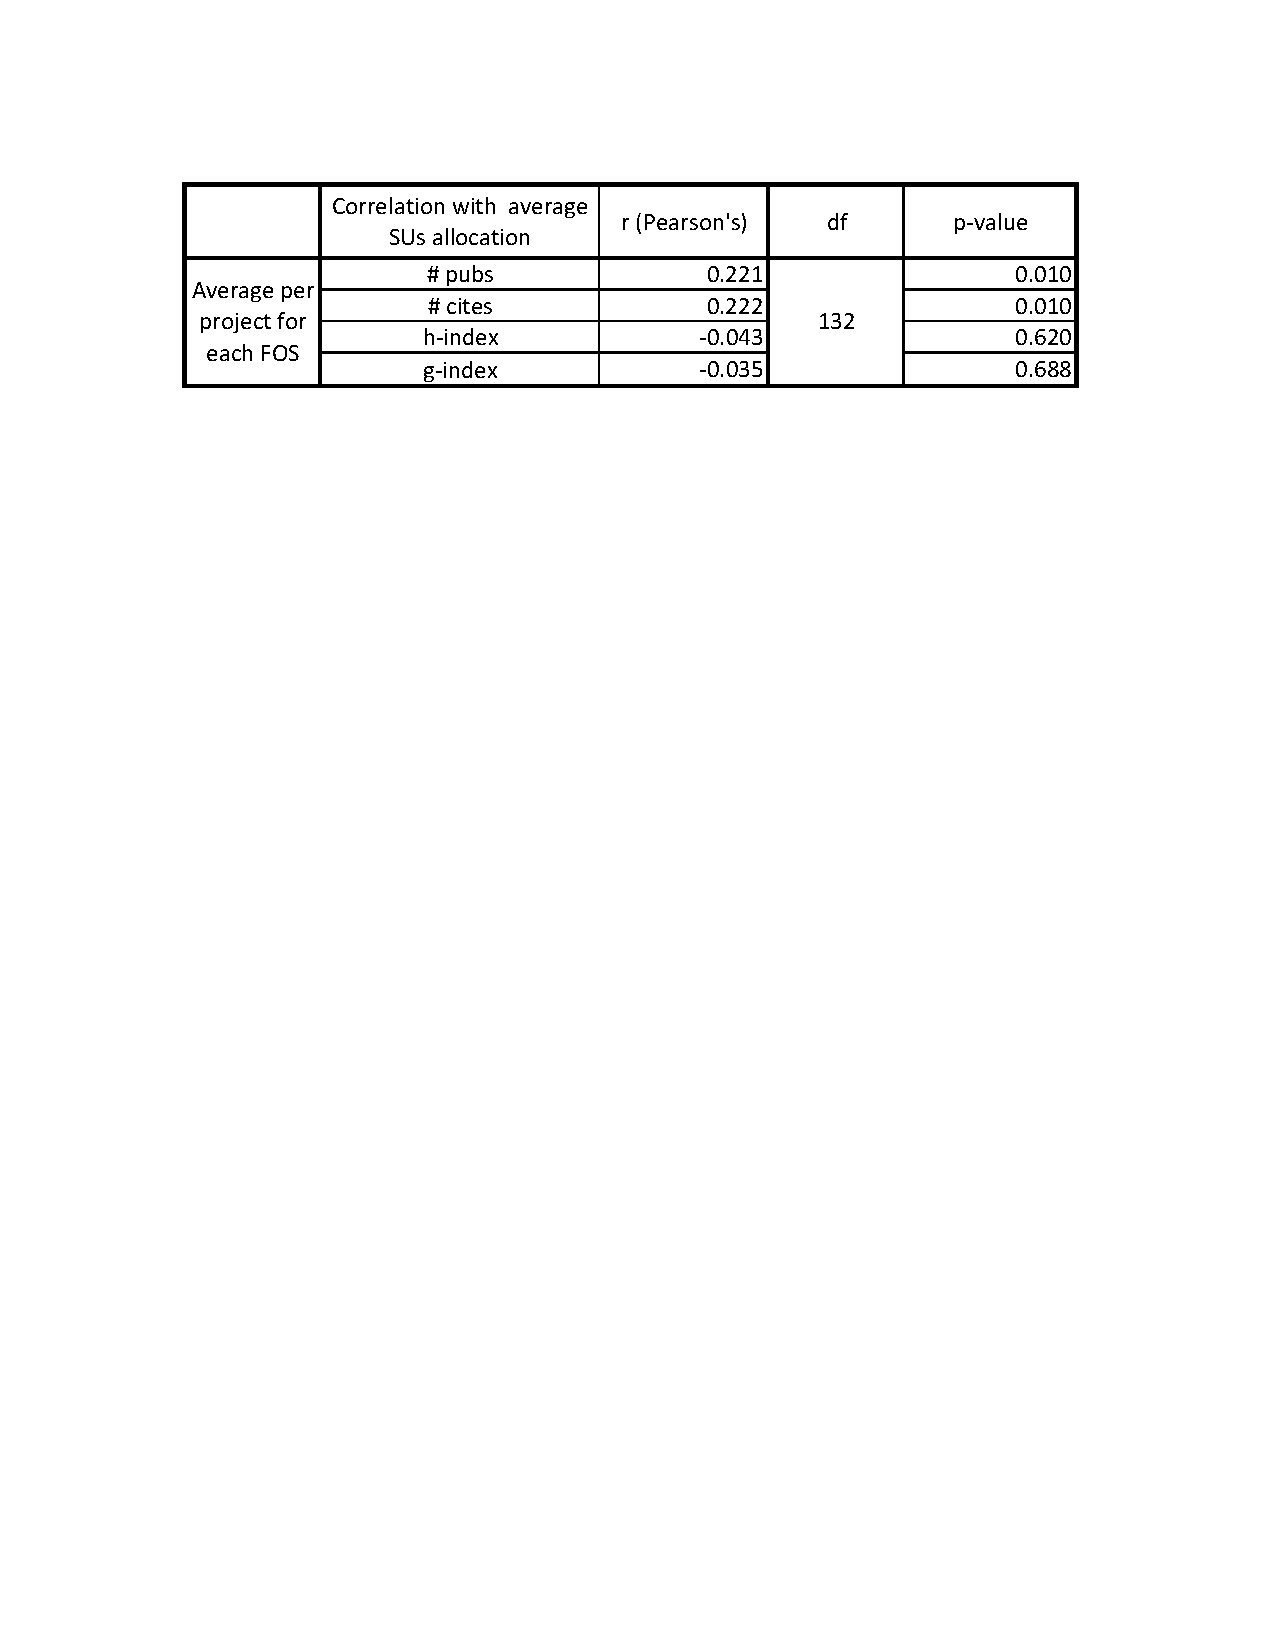
\includegraphics[width=1.0\columnwidth]{images/metrics_alloc_r_fos.pdf} 
  \caption{Correlation between average SUs allocated vs the average impact metrics (by projects) for each FOS}\label{F:metrics-alloc-r-fos} 
\end{table} 
 
As we see, the size of FOS significantly affects the impact as well as the allocations (for h-index as in Figure \ref{F:hindexalloc-vs-nprojects-fos-trended}). We can eliminate this effect by comparing the average by project values within each FOS, as shown in Figure \ref{F:metrics-vs-alloc-avg-log-fit}, while Table \ref{F:metrics-alloc-r-fos} has the values. It shows the weak correlation of per project based metrics vs SUs for the number of publications and citations, which is actually not significantly different than the result from Table \ref{F:metrics-alloc-r}. We didn't observe any correlation between allocation and h-index or g-index. This is probably caused by the fact that these two metrics does not work well when being averaged as they are not cumulative or additive values. 
 
\begin{figure}[!htb] 
  \centering 
    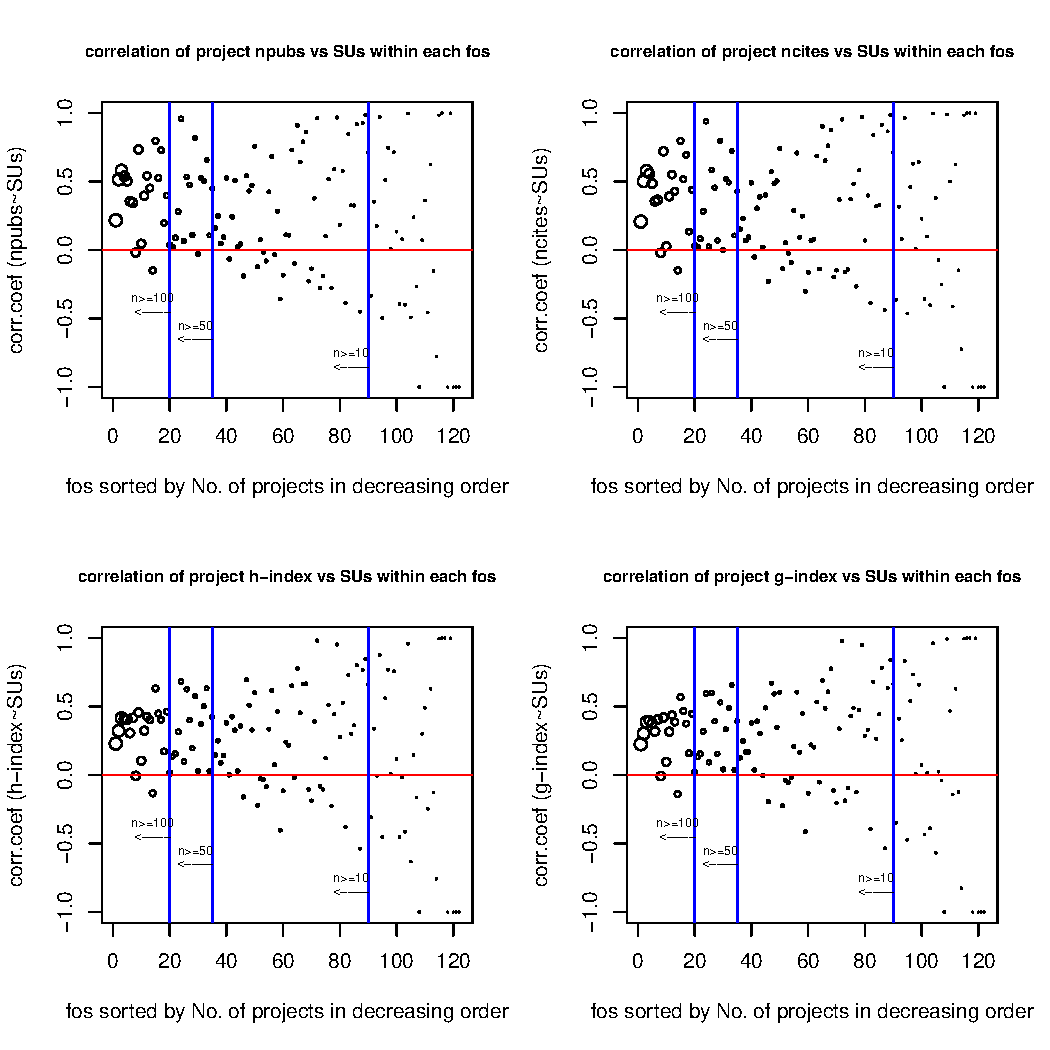
\includegraphics[width=1.0\columnwidth]{images/06_corr_metrics_vs_alloc_proj_by_fos.pdf} 
  \caption{Correlations of impact metrics vs SUs on project level for each FOS}\label{F:corr-metrics-vs-alloc-proj-by-fos} 
\end{figure} 
 
However as shown in Figure \ref{F:corr-metrics-vs-alloc-proj-by-fos}, within each FOS, the project level metrics vs SUs correlations are typically a bit higher especially for those large size FOS's. With increasing size of the FOS (n=10, n=50, and n=100 are denoted as vertical lines), the correlation appears positively higher and more significant. This suggests that for most FOS, impact metrics for a project do have a positive correlations with SUs allocated to the project. Also by investigating the individual data points, we can see in which FOS this correlation appears much stronger, while for some others there is no correlation at all.
 
%\begin{figure}[!htb] 
%  \centering 
%    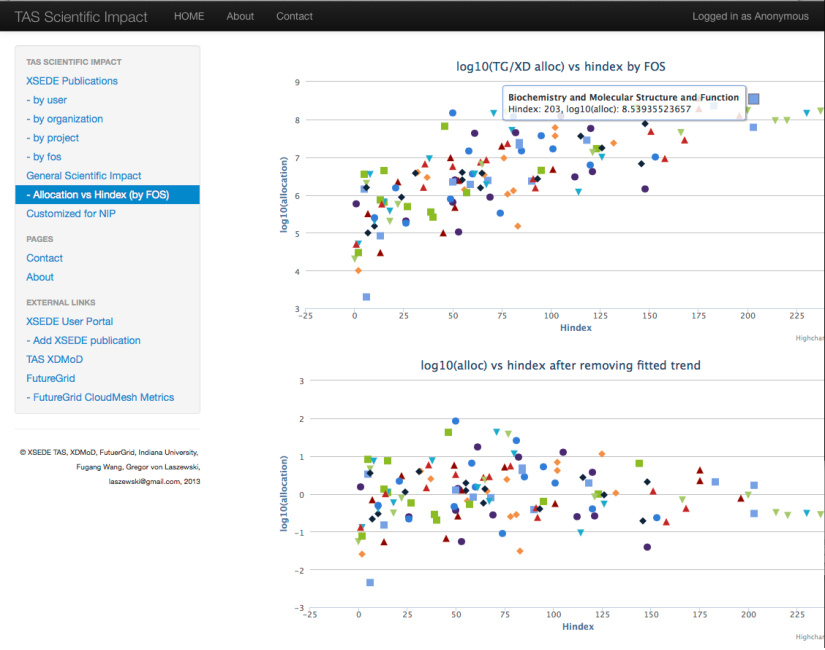
\includegraphics[width=1.0\columnwidth]{images/fig2.pdf} 
%  \caption{fig2.}\label{F:fig2} 
%\end{figure} 
 
%\begin{figure}[!htb] 
%  \centering 
%    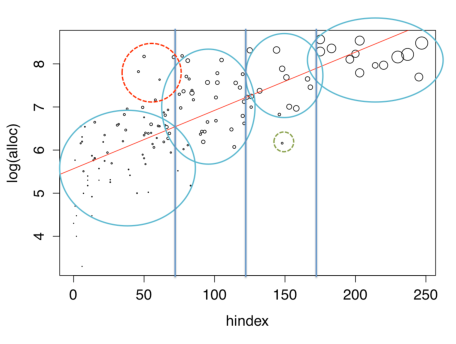
\includegraphics[width=1.0\columnwidth]{images/fig4.pdf} 
%  \caption{fig4.}\label{F:fig4} 
%\end{figure} 
 
%\begin{figure*}[!htb] 
%  \centering 
%    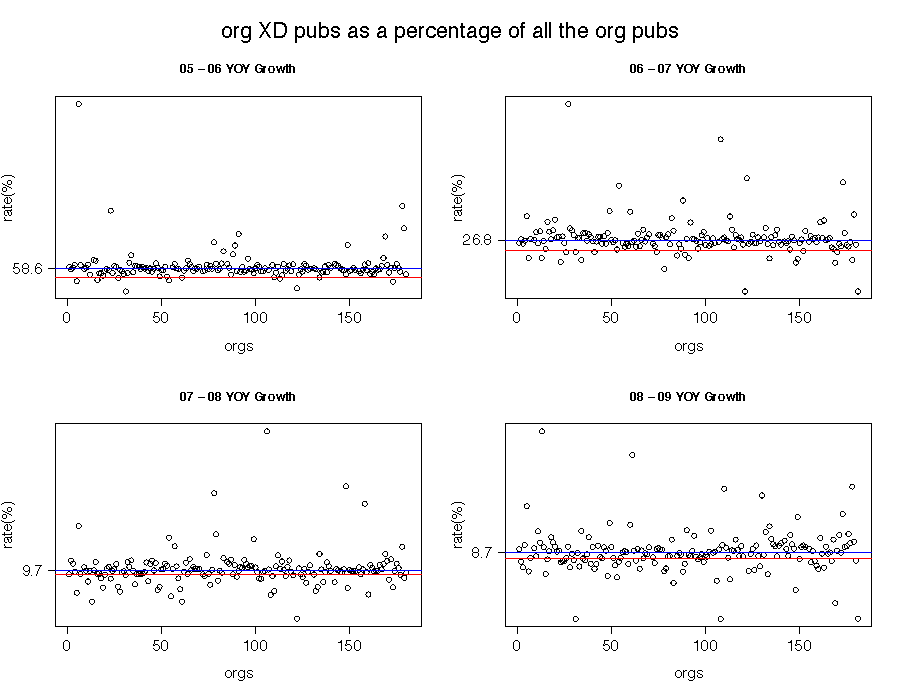
\includegraphics[width=1.0\textwidth]{images/fig5.pdf} 
%  \caption{fig5.}\label{F:fig5} 
%\end{figure*} 
 
% from previous summary report 
 
%\begin{figure}[!htb] 
%  \centering 
%    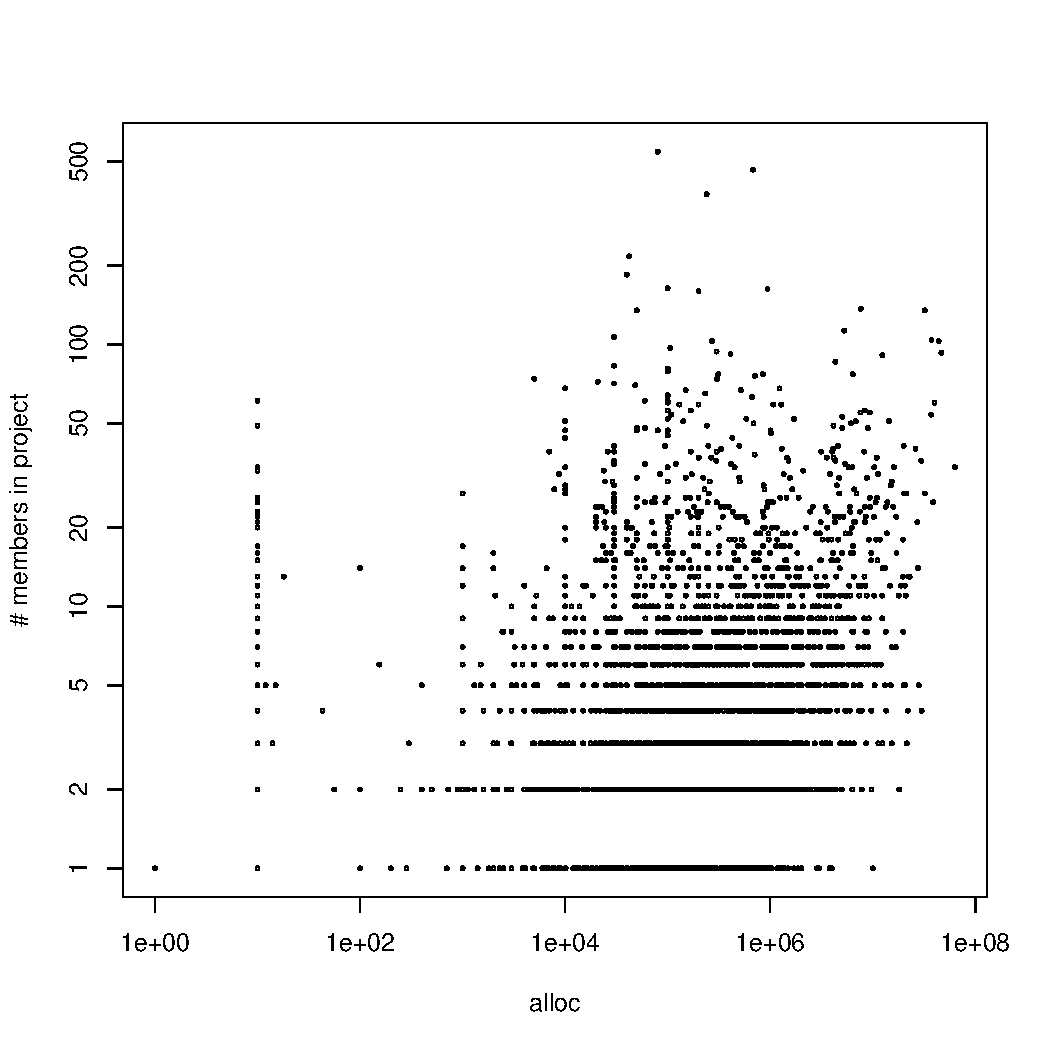
\includegraphics[width=1.0\columnwidth]{images/02_nmembers_vs_alloc_proj.pdf} 
%  \caption{fig3.}\label{F:nmembers-vs-alloc-proj} 
%\end{figure} 
 
%\begin{figure}[!htb] 
%  \centering 
%    \includegraphics[width=1.0\columnwidth]{images/05_alloc_vs_nprojects_fos_trended.pdf} 
%  \caption{fig3.}\label{F:alloc-vs-nprojects-fos-trended} 
%\end{figure} 
 
%\begin{figure}[!htb] 
%  \centering 
%    \includegraphics[width=1.0\columnwidth]{images/05_hindex_vs_nprojects_fos_trended.pdf} 
%  \caption{fig3.}\label{F:hindex-vs-nprojects-fos-trended} 
%\end{figure} 
 
%\begin{figure}[!htb] 
%  \centering 
%    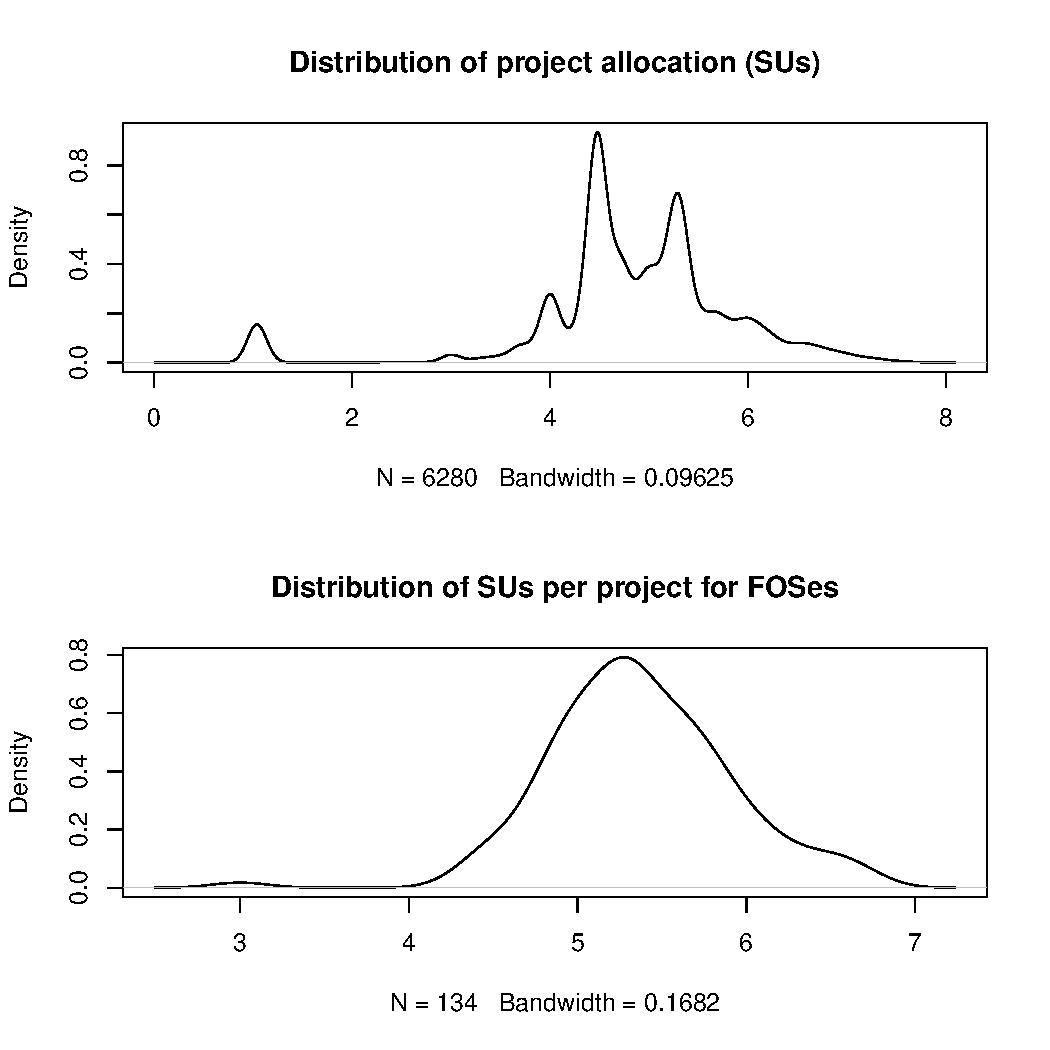
\includegraphics[width=1.0\columnwidth]{images/07_density_alloc.pdf} 
%  \caption{fig3.}\label{F:density-alloc} 
%\end{figure} 
 
%\begin{figure}[!htb] 
%  \centering 
%    \includegraphics[width=1.0\columnwidth]{images/07_density_alloc_fos_avg_by_nprojs.pdf} 
%  \caption{fig3.}\label{F:density-alloc-fos-avg-by-nprojs} 
%\end{figure} 
 
%\begin{figure}[!htb] 
%  \centering 
%    \includegraphics[width=1.0\columnwidth]{images/07_density_alloc_proj.pdf} 
%  \caption{fig3.}\label{F:density-alloc-proj} 
%\end{figure} 
 
 
%\section{Evaluation} 
 
\section{Discussion and Ongoing Work} \label{S:conclusion}
 
This paper does not yet address the name ambiguity issue, which deserves dedicated research and in fact extensive research has been carried out on this issue. The root cause of this issue is that the metadata of the publications simply does not include enough information to distinguish similar names that can be uniquely associated to XSEDE user names. This is not a problem specific to our study but for the automated bibliometrics analysis in general, e.g., Google Scholar also include false positive publications in user profile but leave it to the user to curate the results to make it more accurate. In the future we will try to tackle the problem based on other available data - field of science, organization, funding data, co-author relationship etc. while conducting unsupervised machine learning techniques like k-means clustering as well as the introduction of a social network graph that analyses the authorship for ambiguity and identifies a likelihood.
 
As the ultimate approach is to let users curate their publication list, we would try to include such assisting processes into the workflow of vetting the papers. One pathway we are currently pursuing is to work with the XSEDE portal team while providing the publication data we have collected as a suggestion service, in the hope to provide more convenient way for users to quickly populate the vetted publications library. 
 
We have also started another similar activity, in which we are attemping to  extract and parse the publication data from past TeraGrid/XSEDE quarterly reports. This data, while not curated on per user basis, do have project level association information and thus could serve quite well for most of our analysis. 
 
Another activity we are conducting is social networking related analysis among publications, users, projects, FOS's, etc. based on citation and co-authorship relations.

\section{Summary}

TBD 
 
%%%%%%%%%%%%%%%%%%%%%%%%%%%%%%%%%%%%%%%%%%%%%%%%%%%%%%%%%%%%%%%%%%%%%% 
% Acknowledgment 
%%%%%%%%%%%%%%%%%%%%%%%%%%%%%%%%%%%%%%%%%%%%%%%%%%%%%%%%%%%%%%%%%%%%%% 
 
%ACKNOWLEDGMENTS are optional 
%\section{Acknowledgments} 
 
\section*{Acknowledgement} 
 
This work is part of the Technology Auditing Service (TAS) project sponsored by NSF under grant number OCI 1025159. 
 
%\clearpage 
 
\bibliographystyle{IEEEtranS} 
%\bibliographystyle{abbrv} 
\bibliography{% 
%bib/references,% 
%bib/vonLaszewski-jabref,% 
%bib/image-refs,% 
%bib/cyberaide-cloud,% 
%bib/python,% 
tas.bib} 
 
\end{document} 
 
 

